\documentclass[11pt]{article}
%%%%%%%%%%%%%%%%%%%%%%%%%%%%%%%%%%%%%%%%%%%%%%%%%%%%%%%%%%%%%%%%%%%%%%%%%%%%%%%
% Packages, Commands and Miscellaneous
%%%%%%%%%%%%%%%%%%%%%%%%%%%%%%%%%%%%%%%%%%%%%%%%%%%%%%%%%%%%%%%%%%%%%%%%%%%%%%%

%%%=== PART 1: Packages
\usepackage{amsfonts, amsmath, amssymb}
\usepackage[toc,page]{appendix}
\usepackage{bbm}                              %% for indicator function notation
\usepackage{enumitem}                         %% for customising bullet point lists
\usepackage{float, graphicx, svg, subcaption}
\usepackage{hyperref}                         %% for in-document references
\usepackage[utf8]{inputenc}                   %% for compiler to interpret .tex file
\usepackage{setspace}                         %% for setting vspace between sentences
\usepackage{tikz}                             %% for drawing Bayesian networks
\usepackage{tcolorbox}
\usepackage{xcolor}

\usepackage[pass]{geometry} %% for the minimisation of margins
\newlength\DX
\DX=3.0in
\paperwidth=\dimexpr\paperwidth-\DX\relax
\hoffset=\dimexpr\hoffset-.5\DX\relax
\newlength\DY
\DY=2.8in
\paperheight=\dimexpr\paperheight-\DY\relax
\voffset=\dimexpr\voffset-.5\DY-.5\footskip\relax

%%%=== PART 2: Commands
\newcommand{\D}{\mathcal{D}}
\newcommand{\E}{\mathbb{E}}
\newcommand{\R}{\mathbb{R}}
\newcommand{\X}{\mathbf{X}}
\newcommand{\Z}{\mathbf{Z}}

\newcommand{\x}{\mathbf{x}}
\newcommand{\z}{\mathbf{z}}

\newcommand{\REVIEW}{\textcolor{purple}{\textbf{REVIEW: }}}
\newcommand{\TODO}{\textcolor{red}{\textbf{TODO: }}}
\newcommand{\IMPROVE}{\textcolor{myYellow}{\textbf{IMPROVE: }}}

\renewcommand{\l}{\left}
\renewcommand{\r}{\right}

%%%=== PART 3: Miscellaneous
\captionsetup{labelfont=bf}

\DeclareMathOperator*{\argmax}{arg\,max}
\DeclareMathOperator*{\argmin}{arg\,min}

\definecolor{myDarkBlue} {RGB}{ 15, 61,138}
\definecolor{myGreen}    {RGB}{  0,128,128}
\definecolor{myLightBlue}{RGB}{173,216,230}
\definecolor{myLightRed} {RGB}{255, 99, 71}
\definecolor{myYellow}   {RGB}{255,165,  0}


\begin{document}

% title
\begin{center}
\HRule\\[0.6cm]
{\huge\bfseries Machine Learning Explainers}\\[0.2cm]
\textbf{Last updated:} \today\\
\HRule\\[0.6cm]
\end{center}

% abstract
\begin{abstract}
    \noindent Summaries of a bunch of machine/deep learning-related topics. My main motive in writing this is as a reminder for future me.
\end{abstract}

% table of contents
\setcounter{tocdepth}{2}{\footnotesize\tableofcontents}

% title page number not counted
\thispagestyle{empty}
\setcounter{page}{0}
\newpage

% intro
\section{Introduction}

I think of machine learning as the discipline of studying methods of learning parameterised models over from data. What makes machine learning fun is the stupidly high rate of improvement of the discipline since 2012. At their core, many methods boil down to statistically-principled things, like maximum likelihood, \dots. The fact that this is possible to at least a small extent isn't too surprising, but, nowadays, this is possible to the extent of being able to do things like input natural language to output a photo-realistic image described by said input. Why is this possible? The more I've learned, the more I'm amazed that our methods work as well as they do. Take denoising diffusion models for image generation. It effectively learns to transform randomly sampled Gaussian noise into something convincingly belonging to the distribution pertainintg to the data that the model was trained on. So if I train such a model on a large dataset of images of cats then it learns to transform Gaussian noise into new images of cats that are sufficiently distinct from those it was trained on. That is, such models do not necessarily need to overfit to be able to output samples convincingly belonging to the target distribution. Why are diffusion, flow-based models, GANs, VAEs, probabilistic circuits or attention-based models so effective? It's sometimes hard to believe, even after working with some of these architectures extensively and understanding them in detail.

% thoughts on reasoning
\section*{Thoughts on reasoning}

As a term, machine learning is used almost interchangeably with AI as of now (summer of 2024). AI isn't particularly well-defined in itself, even in academic settings, so its use in day-to-day things, like the news, can be confusing. I think of machine learning as what's written above, effectively in line with statistical learning theory. I'm not sure how I would define AI in a way that'd satisfy most. Maybe the discipline of studying things that can `reason', as a human does, given some agreeable notion of `reasoning'. A common issue found in discussions surrounding this topic is that a definition of `reasoning' is left out. In fairness, it's a tricky thing to define precisely.

Right now, I'm unaware of any machine learning model that can `reason' by any agreeable notion of the term. Let's say that GPT-4o concludes that a continuous real-valued function $f:\R\rightarrow\R$ has a root in some interval $(a, b)$ using the intermediate value theorem (IVT) by noting that $f(a)<0$ and $f(b)>0$. Is this `reasoning' or do we instead brush this off as the model having been trained on a bunch of examples of the use of IVT? Does it understand what it's concluding? As of right now I'd say that it doesn't. This of course isn't something unique to IVT — we can construct many such examples. What I think makes IVT interesting is that we can effectively express what it means to understand it as a human. I'd say that the distinction between ChatGPT's `understanding' here and a human's is that a human knows that if they trace their finger on a piece of paper starting from the bottom half, crossing a horizontal line cutting through the middle, to the top half of the page without taking their finger off the paper then their finger must have touched the horizontal line at some point, i.e. the function must have intersected the $x$-axis during this continuous traversal. I believe that humans understand this due to just experiencing the real world. You don't need any mathematical training to know and, more importantly, understand `why' your finger crosses through this horizontal line on the page. I'm certain that current GPT models do not `understand' the IVT in this way, or really any way that isn't purely formally mathematical.

A separate but related question is to what extent it matters that a model `understands' how it arrives at its conclusions. Somewhat in the same way that it doesn't matter that a calculator has no inherent idea of why it outputs 6 when you input $3\cdot2$. Maybe 50 years from now we'll be well-taken care of by a fleet of machine learning-based robots and we'll still complain that they aren't truly capable of reasoning like us.

% supervised learning
\section{Supervised Learning}

Supervised learning algorithms are a class of machine learning algorithms in which a model learns some relationship between model variables and output variables by being shown concrete examples of what a given input (pertaining to the model variables) should yield as output. These model and output variables can be continuous or discrete in nature but usually it's a mix.

An example of a task which supervised learning is appropriate for includes regression predicting life expectancies of a poulation given features such as the population's height, age, BMI etc. You can think of regression tasks as those where the output of the model should belong to some continuously distributed space. Other than regression, the other vanilla supervised learning task is binary or multi-class classification. Well known examples of binary classification include whether or not a given passenger survived the titanic wreck given their ticket class, sex, age, port of embarkation and a ton more. The bread and butter example of multi-class classification is handwritten digit recognition. It's amazing that something difficult as recently as 2005 is trivial now for various levels of machine learing understanding.

Other than the types of tasks which we consider in this section, it's worth mentioning how we deal with our data in general. In training a model on some dataset, we need some idea of how well the model generalises to new data. This is done by splitting the given dataset $\D$ into a training set $\Dtrain$ and a testing set $\Dtest$. How exactly this split is done depends on the task at hand but an example is 50/50 uniformly randomly splitting the original dataset $\D$ — chronologically or not. It can be important that this is done uniformly randomly. For example, if one is tackling a binary classification task and $\D$ consists of $1000$ samples with $500$ belonging to class 1 and $500$ belonging to class 2 then it's important that one does not split in a way that causes egregiously imbalanced representations of these classes. Training a model on $500$ samples of class 1 then testing it on $500$ samples of class 2 wouldn't make much sense. Similar idea for regression tasks but with ensuring a reasonable balance in representation of values belonging to given intervals corresponding to the output space. With a reasonable split we train the model on $\Dtrain$. It is all the model knows — $\Dtrain$ is the model's universe. After training, we measure the model's ability to generalise to new samples belonging to the same underlying distribution by seeing how well it performs with respect to the samples in $\Dtest$. Essentially comparing its output given some sample to the ideal/true output value of said sample. Things get a bit more fancy when we consider cross-validation but that'll come later.

% linear regression
\subsection{Linear Regression}

\textbf{Note:} There are some pieces of literature that define linear regression models as regression models that are linear in their parameters. By this definition, linear regression, as a term, would encompass polynomial regression models and other regression models with non-linear basis functions so long as the model is linear in its parameters. This confuses me as `linear regression' most often refers to models that fit a hyperplane to the data.

In fairness, from what I understand, using the least squares method derived below for all such regression models linear in their parameters is viable.\\

\noindent Perhaps the simplest example of supervised learning is linear regression. Suppose we are given a dataset $\D=\{(\x_i,y_i)\}_{i=1,\dots,2n}$ where
$$
\x_i=(x_{i,1},\dots,x_{i, p})\in \Omega_{X_1}\times\dots\times \Omega_{X_p}=:\OX\subseteq\R^p
$$
are the feature values of the $i^{\text{th}}$ sample and $y_i\in \OY\subseteq\R$ is the corresponding output. The reason I chose $|\D|=2n$ is that it results in being able to 50/50 split $\D$ into $\Dtrain$ and $\Dtest$ with $|\Dtrain|=|\Dtest|=n$. A linear regression models fits a linear function (in the parameters)
\begin{align*}
    f_{\theta}:\OX&\rightarrow \Omega_Y\\
    \x&\mapsto
    \theta^{\T}
    \begin{bmatrix}
        1\\
        \x
    \end{bmatrix}
    =
    \theta_0+\theta_1x_1+\dots+\theta_px_p    
\end{align*}
where $\theta=(\theta_0,\theta_1\dots,\theta_p)\in\R^{p+1}$ are the model parameters, i.e. the values we can tweak to our heart's desire until the corresponding model is sufficiently well according to some metric. Some people refer to the paramter $\theta_0$, which dictates the elevation of the hyperplane corresponding to $f_{\theta}(\x)=0$, as the bias of the model which I find very confusing as there are a bunch of other intended meanings of the term `bias' in statistics and machine learning. I prefer to refer to it as the elevation. Anyway, once such a linear function has been fit, given feature values $\tilde{\x}\in\OX$ we can predict the corresponding output as $\tilde{y}=f_{\theta}(\tilde{\x})$.

An intuitive approach to finding the `optimal' parameters for a linear regression model, which we denote by $\thetaOpt$, is to split $\D$ into training and testing datasets $\Dtrain$ and $\Dtest$ (each consisting of $n$ sample in our case) and minimising some pre-determined loss function of said parameters over $\Dtrain$. Essentially, minimising something like
$$
\text{Loss}(\theta)=\sum_{i=1}^nd(f_{\theta}(\x_i), y_i)
$$
where $f_{\theta}(\x_i)$ is the model's prediction for feature values $\x_i$ and $d:Y\times Y\rightarrow\R_{\geq0}$ is some metric on the set of possible output values and itself. Said loss function gives one an idea of how well $\theta$ fits the true underlying relationship which we wish to model. A common choice for the loss function is the mean square error
$$
\text{MSE}(\theta)=\sum_{i=1}^n(y_i-f_{\theta}(\x_i))^2
$$
which pertains to taking $d(f_{\theta}(\x_i), y_i)=(y_i-f_{\theta}(\x_i))^2$. I'll still refer to it as the `mean' square error, even though I don't divide by $n$, simply because minimising it as written above is equivalent to minimising the same expression with division by $n$ included — it's mostly a notational convenience thing. So in our case, we wish to find
$$
\thetaOpt=\argmin_{\theta\in\R^{p+1}}\l[\sum_{i=1}^n(y_i-f_{\theta}(\x_i))^2\r].
$$

\noindent We know that in the context of linear regression, the optimal paramters $\thetaOpt$ are typically taken to be those which minimise the mean square error over $\Dtrain$ but how do we actually compute $\thetaOpt$? This could be done through numerical methods, which is often the case in machine learning, e.g. using gradient descent in computing the optimal parameters of a logistic regression model, but linear regression has a closed form solution. This is pretty cool since it's not so common for such closed form solutions to exist. The informal method which I use to remember the closed form solution for the optimal paramters of a linear regression model is
$$
X\thetaOpt=y \implies X^{\T}X\thetaOpt=X^{\T}y \implies \thetaOpt=(X^{\T}X)^{-1}X^{\T}y.
$$
In practice, if this matrix $X^{\T}X$ is singular then just add some small values to its diagonal. That is, instead compute
$$
\thetaOpt=(X^{\T}X+\delta I)^{-1}X^{\T}y
$$
for some small $\delta\in\R$. That said, what's given above is not rigorous, so let's derive it. Note that
\begin{align*}
    \text{MSE}(\theta)
    &=
    \sum_{i=1}^n(y_i-f_{\theta}(\x_i))^2\\
    &=
    \begin{bmatrix}
        y_1-f_{\theta}(\x_1) & \cdots & y_n-f_{\theta}(\x_n)
    \end{bmatrix}
    \begin{bmatrix}
        y_1-f_{\theta}(\x_1)\\
        \vdots\\
        y_n-f_{\theta}(\x_n)
    \end{bmatrix}\\
    &=(y-X\theta)^{\T}(y-X\theta)\\
    &=||y-X\theta||^2
\end{align*}
where
$$
y
=
\begin{bmatrix}
    y_1\\
    \vdots\\
    y_n
\end{bmatrix}
\in\R^n,
X
=
\begin{bmatrix}
    1 & x_{1,1} & \cdots & x_{1,p}\\
    \vdots & \vdots & \ddots & \vdots\\
    1 & x_{n,1} & \cdots & x_{n,p}
\end{bmatrix}
\in\R^{n\times (p+1)},
\theta
=
\begin{bmatrix}
    \theta_0\\
    \theta_1\\
    \vdots\\
    \theta_p
\end{bmatrix}
\in\R^{p+1}
$$
and $x_{i,j}$ denotes the $j$th element of the $i^{\text{th}}$ sample. To find the minimiser(s) of $\text{MSE}(\theta)$, i.e. the optimal parameters $\thetaOpt$, we compute its gradient with respect to $\theta$, set it to $0$ and solve for $\thetaOpt$. This of course only works when our function is both differentiable and convex, which is the case here. To see convexity, simply compute the Hessian of $\text{MSE}(\theta)$ and see that it is semi-positive definite. On that note, we have
\begin{align*}
    \nabla\text{MSE}(\theta)
    &=
    \nabla||y-X\theta||^2\\
    &=
    \nabla(y-X\theta)^{\T}(y-X\theta)\\
    &=
    \nabla\l[\theta^{\T}X^{\T}X\theta-\theta^{\T}X^{\T}y-y^{\T}X\theta+y^{\T}y\r]\\
    &=
    \nabla\l[\theta^{\T}X^{\T}X\theta-2y^{\T}X\theta+y^{\T}y\r]\\
    &=
    2X^{\T}X\theta-2X^{\T}y
\end{align*}
and so the optimiser $\thetaOpt$ is given by
$$
\thetaOpt=(X^{\T}X)^{-1}X^{\T}y.
$$

\subsubsection{Statistical Motivation}

This idea of minimising the mean square error of the model over $\Dtrain$ even has some rigorous statistical motivation. Assume that the residuals corresponding of the model's output over $\Dtrain$ are independent and identically normally distributed with mean 0. That is, assume
$$
e_i
=
y_i-f_{\theta}(\x_i)\sim\N(0, \sigma^2)
$$
for $i=1,\dots,n$ are i.i.d. This assumption is reasonable in practice via the CLT. Since $f_{\theta}(\x_i)$ is a constant, we have $y_i|\x_i\sim\N(f_{\theta}(\x_i), \sigma^2)$ and so
$$
\P(y_i|\x_i;\theta)=\frac{1}{\sqrt{2\pi}\sigma}\exp\l(-\frac{(y_i-f_{\theta}(\x_i))^2}{2\sigma^2}\r).
$$
By the law of maximum likelihood\footnote{maximum likelihood link}, the maximum likelihood estimator $\theta_{\text{MLE}}$ for the parameters of our linear regression model is that which maximise our log-likelihood. That is,
\begin{align*}
    \theta_{\text{MLE}}&=\argmax_{\theta}\l[\log\l(\prod_{i=1}^n\P(y_i|\x_i;\theta)\r)\r]\\
    &=\argmax_{\theta}\l[\sum_{i=1}^n\log(\P(y_i|\x_i;\theta))\r]\\
    &=\argmax_{\theta}\l[n\log\l(\frac{1}{\sqrt{2\pi}\sigma}\r)-\frac{1}{2\sigma^2}\sum_{i=1}^n(y_i-f_{\w,b}(\x_i))^2\r]\\
    &=\argmin_{\theta}\l[\sum_{i=1}^n(y_i-f_{\w,b}(\x_i))^2\r].
\end{align*}
As such, the maximum likelihood estimator of the parameters of a linear regression model are precisely those which minimise the mean square error of the model over $\Dtrain$.

\subsubsection{Example}

\begin{table}[ht]
    \begin{center}
        \begin{tabular}{c|c||c}
            Age (years) & BMI (kg/m$^2$) & Cholesterol (mg/dL)\\
            \hline
            \hline
            25 & 22.5 & 180 \\
            30 & 24.0 & 190 \\
            35 & 26.5 & 210 \\
            40 & 28.0 & 220 \\
            45 & 29.5 & 240 \\
            50 & 30.0 & 250 \\
            55 & 31.5 & 260 \\
            60 & 32.0 & 270 \\
            65 & 33.5 & 280 \\
            70 & 34.0 & 290 \\
            \hline
        \end{tabular}
    \end{center}
    \vspace{-15pt}
    \caption{Patient data pertaining to their age, BMI and cholesterol levels.}
    \label{tab:lin_reg_example}
\end{table}

\noindent Suppose we are given the dataset illustrated in \autoref{tab:lin_reg_example} pertaining to a set of patients' ages, BMIs and cholesterol levels and that we would like to predict the cholesterol levels of some other set of patients based on their ages and heights. In this context we have two features, age and BMI, which will correspond to the parameters $\theta_1$ and $\theta_2$ respectively. As such, our model's output function will be of the form
$$
f_{\theta}(\x)=\theta_0+\theta_1x_1+\theta_2x_2
$$
where $x_1$ and $x_2$ correspond to the input sample patient's age and BMI level respectively. Before fitting a linear regression model to our dataset, it's a good idea to see if a linear underlying relationship exists in the first place. To do this, we can plot the given dataset to obtain \autoref{fig:not_at_all_the_same}.

\begin{figure}[ht]
    \centering
    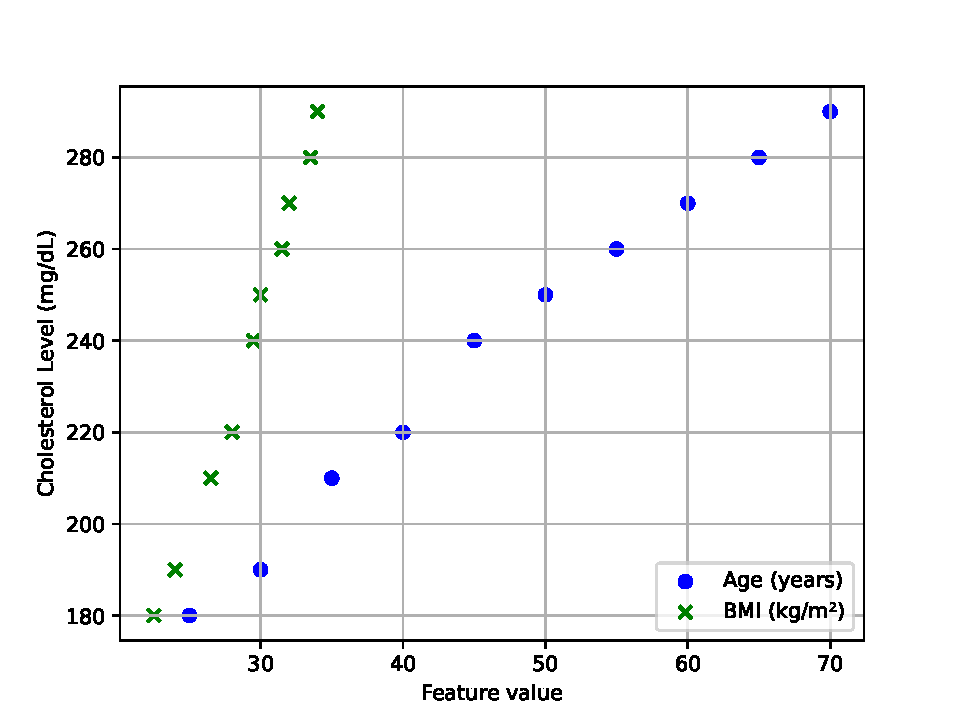
\includegraphics[width=0.49\columnwidth]{./figures/supervised_learning/lin_reg_example/age_and_bmi_vs_cholesterol.pdf}
    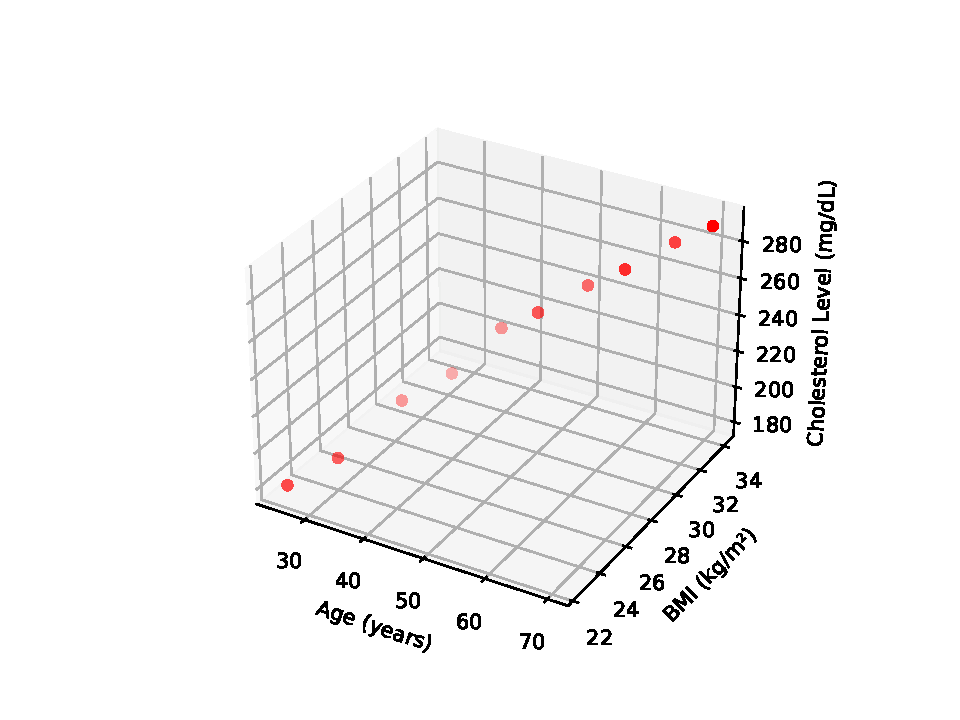
\includegraphics[width=0.49\columnwidth]{./figures/supervised_learning/lin_reg_example/age_vs_bmi_vs_cholesterol.pdf}
    \caption{Each feature against the output (left) and the dataset in the feature space (right).}
    \label{fig:not_at_all_the_same}
\end{figure}

\noindent Looks sufficiently linear to me. We'll split the dataset into training and testing datasets via \autoref{tab:lin_reg_example_train} and \autoref{tab:lin_reg_example_test}.
\begin{table}[ht]
    \begin{center}
        \begin{minipage}{0.49\textwidth}
            \begin{center}
                \begin{tabular}{c|c||c}
                    Age & BMI & Cholesterol\\
                    \hline
                    \hline
                    25 & 22.5 & 180 \\
                    35 & 26.5 & 210 \\
                    45 & 29.5 & 240 \\
                    55 & 31.5 & 260 \\
                    65 & 33.5 & 280 \\
                    \hline
                \end{tabular}
                \caption{Training dataset.}
                \label{tab:lin_reg_example_train}
            \end{center}
        \end{minipage} \hfill
        \begin{minipage}{0.49\textwidth}
            \begin{center}
                \begin{tabular}{c|c||c}
                    Age & BMI & Cholesterol\\
                    \hline
                    \hline
                    30 & 24.0 & 190 \\
                    40 & 28.0 & 220 \\
                    50 & 30.0 & 250 \\
                    60 & 32.0 & 270 \\
                    70 & 34.0 & 290 \\
                    \hline
                \end{tabular}
                \caption{Testing dataset.}
                \label{tab:lin_reg_example_test}
            \end{center}
        \end{minipage}
    \end{center}
\end{table}
Since $\Dtrain$ consists of only five samples, it's feasible to write out the optimal parameters $\thetaOpt$ by hand. We have
$$
y=
\begin{bmatrix}
    180\\
    210\\
    240\\
    260\\
    280\\
\end{bmatrix},
\hspace{10pt}
X=
\begin{bmatrix}
    1 & 25 & 22.5 \\
    1 & 35 & 26.5 \\
    1 & 45 & 29.5 \\
    1 & 55 & 31.5 \\
    1 & 65 & 33.5
\end{bmatrix}
$$
from which we obtain
$$
\thetaOpt
=
\l(X^{\T}X\r)^{-1}X^{\T}y
=
\begin{bmatrix}
    25.68\\
    0.94\\
    5.79
\end{bmatrix}
$$
which corresponds to
$$
f(x_1,x_2)=25.68+0.94x_1+5.79x_2.
$$

What's nice about such a low-dimensional problem like this is that visualising the loss landscape is relatively doable. We have three parameters so I'll fix $\theta_0=25.68$ and plot $\theta_1$ and $\theta$ against 
$$
\text{MSE}(25.68, \theta_1, \theta_2)
=
\sum_{i=1}^5 (y_i-25.68-\theta_1\x_{1,1}-\theta_2\x_{1,2})^2
$$
where the sum is taken over the training data $\{(\x_i,y_i)\}_{i=1,\dots,5}$.

As for how well the model performs, its MSE on $\Dtrain$ is $1.26$ and its MSE on $\Dtest$ is $12.24$. In this case, such a difference is fine. To get a visual on how well the model does on the training and testing sets, consider \autoref{fig:lin_reg_example_on_train_and_test}. I should improve these at some point.

\begin{figure}[ht]
    \centering
    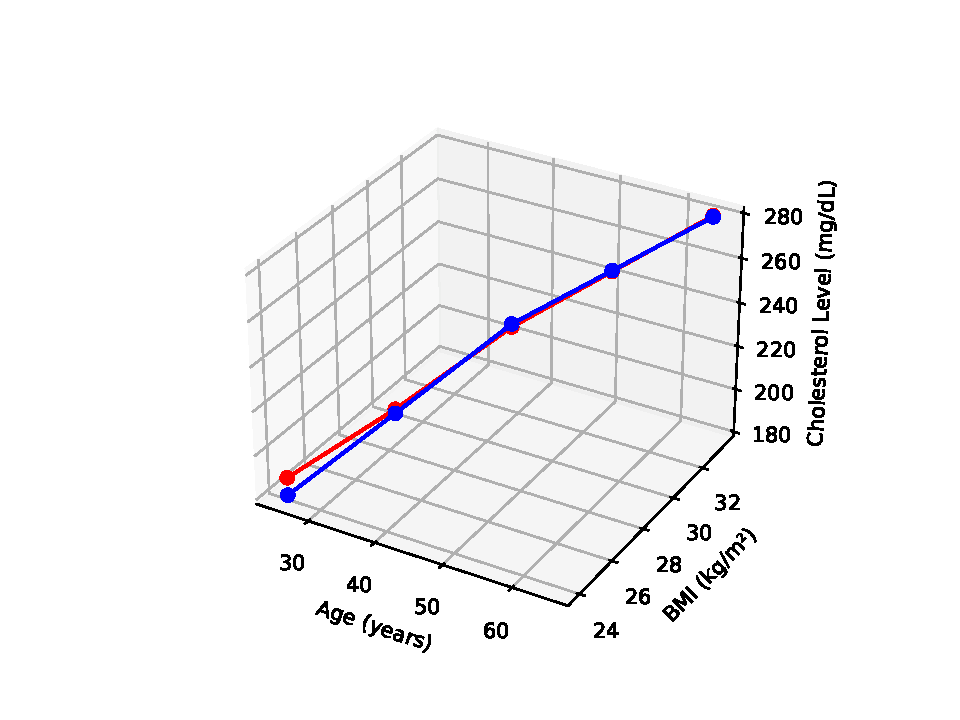
\includegraphics[width=0.49\columnwidth]{./figures/supervised_learning/lin_reg_example/model_predicts_train.pdf}
    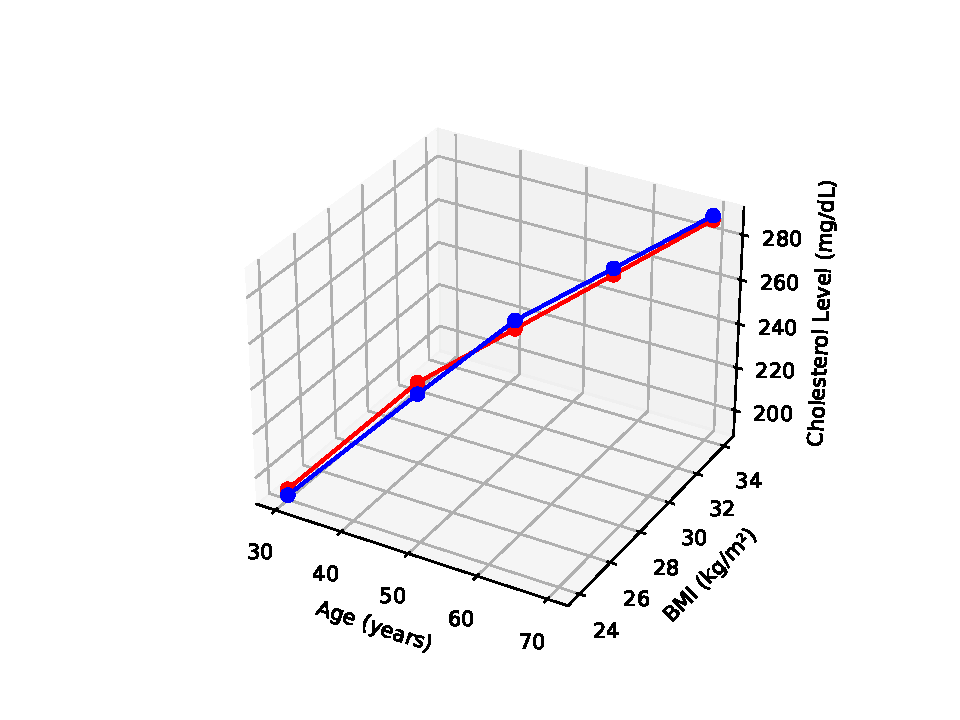
\includegraphics[width=0.49\columnwidth]{./figures/supervised_learning/lin_reg_example/model_predicts_test.pdf}
    \caption{Model performance on the training set (left) and testing set (right).}
    \label{fig:lin_reg_example_on_train_and_test}
\end{figure}

\begin{tcolorbox}[colback=c2]
    \textbf{Funny misuse of linear regression: Momentous sprint at the 2156 Olympics?}
    \vspace{10pt}

    The following is taken from an answer on Quora\footnote{\url{https://qr.ae/pslbEN}} (the top comment is worth reading) based on a paper\footnote{\url{https://www.ncbi.nlm.nih.gov/pmc/articles/PMC3173856/}} published in Nature. Related\footnote{\url{https://xkcd.com/1007/}}.
\end{tcolorbox}

\subsubsection{Regularisation}
The most well known methods of regularisation in the context of regression are Lasso and Ridge regression. These are also known as L1 and L2 regularisation. They are motivated very nicely using Bayesian arguments. L1 regularisation corresponds to a Laplace prior and L2 to a Gaussian prior.

\subsubsection{$R^2$ value}
\dots

\begin{tcolorbox}[colback=c2]
    \textbf{Assumption of normally distributed residuals}
    \vspace{10pt}

    Central limit theorem to the rescue!\footnote{\url{https://en.wikipedia.org/wiki/Central\_limit\_theorem\#Regression}} ``Regression analysis, and in particular ordinary least squares, specifies that a dependent variable depends according to some function upon one or more independent variables, with an additive error term. Various types of statistical inference on the regression assume that the error term is normally distributed. This assumption can be justified by assuming that the error term is actually the sum of many independent error terms; even if the individual error terms are not normally distributed, by the central limit theorem their sum can be well approximated by a normal distribution."\\

    Another good link: \url{https://stats.stackexchange.com/a/12266}.
\end{tcolorbox}

\subsubsection{Terminology}

Nowadays, regression models are those which predict a value belonging to some continuous space but where did it come from? In 1886, Francis Galton authored ``Regression Towards Mediocrity in Hereditary Stature'' which is where the `regression towards the mean' term comes from. Galton noticed that tall father's have short sons, short fathers have tall sons and average height fathers have average height sons. Taken from a Stack Exchange comment: ``Galton derived a linear approximation to estimate a son's height from the father's height in that paper. His equation was fitted so an average height father would have an average height son, but a taller than average father would have a son that is taller than average by 2/3 the amount his father is. Same with shorter than average. This could be argued to be a simple linear regression."

Put mathematically, suppose random variables $X$ and $Y$ are related via $Y=\alpha+\beta X+\epsilon$ where $\alpha,\beta\in\R$ are regression coefficients and $\epsilon$ is noise with mean $0$. Then $\E[Y|X]=\alpha+\beta X$, so if we first normalise to have RVs of mean 0 and variance 1 then we would have $E[Y|X]=\rho X$ where $\rho$ is the correlation coefficient between $X$ and $Y$. Since $|\rho|\leq1$ we know that the expected value of $Y$ is close to the mean than $X$ unless $\rho=1$. So extreme values of $X$ tend to correspond to values of $Y$ that are closer to the mean, i.e. one has regression towards the mean.

To see why this does not apply to all modern `regression' models, consider logistic regression in which one, roughly speaking, predicts probabilities of binary outcomes. In such cases, the dependent variable is binary, so `regressing towards the mean' has no meaningful interpretation.

The `linear' part refers to the output variable being linear in the parameters. This is sometimes confusing in linear regression we typically deal with basis functions that give line-like surfaces (lines, planes, etc.) but we could always have non-linear basis functions. For example, $y=\beta_0+\beta_1 e^x$ is linear in $\beta=(\beta_0,\beta_1)$ but $y=\beta_0+e^{\beta_1}x$ is not. A consequence is that an estimate $\hat{\beta}$ of the model parameters can be written as $\hat{\beta}=\sum_{i=1}^k w_iy_i$ where $w_i$ are the determined weights and $y_i$ are the chosen basis functions.

% how good is good data
\subsubsection{Opportunity to Demonstrate High Quality Data}

Let's say we had perfect data. That is, no noise and samples truly lie on the underlying hyperplane fit. In such a case, if our samples are of the form $(x_1,\dots,x_n,y)\in\R^{n+1}$ then the hyperplanes of interest are $n$-dimensional (assuming independent features?) and each is uniuely identified by $n+1$ distinct points on the plane. So if our data is perfect then bam, all we need is $n+1$ linearly independent samples to perfectly fit the data in the linear regression case.

The idea of course extends to things like polynomial regression, just more points are needed depending on the degree.

% logistic regression
\subsection{Logistic Regression}

While linear regression is the staple example of regression models, its equivalent for binary classification is logistic regression. The name is a bit confusing at first since it's fair to expect that something with the name regression would be used for regression tasks, i.e. predicting something continuously distributed, as opposed to something discrete like binary classification. Logistic Regression essentially applies a logistic (or sigmoid) transformation to the output of our model to introduce a notion of confidence of the classification. Understandably, this transformation maps all outputs to $(0,1)$. This is what makes it regression-like.

Binary classification is the task of assigning one of two classes to some input sample. For example, given some data pertaining to a patient's health, it might be nice to be able to predict whether they are at risk of suffering from a heart attack or not. With this in mind, how does one classify a sample at all? The idea is to fit a hyperplane to the feature space of the distribution which we wish to model. A hyperplane is an $(n-1)$-dimensional object embedded in $n$-dimensional space. So in 2D space, a hyperplane is just a line and in 3D space it's a plane etc. A hyperplane in $(p+1)-$dimensional space consists of the points $(x_1,\dots,x_p)\in\R^p$ which satisfy
$$
\theta_0+\theta_1x_1+\dots+\theta_px_p=0
$$
where $\theta=(\theta_0,\dots,\theta_p)$ are the hyperplane's coefficients and $\x=(1,x_1,\dots,x_p)$ and we can denote the function corresponding to the hyperplane by
$$
f_{\theta}(\x)
=
\theta_0+\theta_1x_1+\dots+\theta_px_p
=
\theta^{\text{T}}\x.
$$
The reason for the additional $1$ appearing at the beginning of $\x$ is similar to as in linear regression: it accounts for the bias term $\theta_0$ and makes notation a lot cleaner. After fitting the parameters of such a hyperplane, we can classify a sample $\x$ according to which side of the hyperplane $f_{\theta}(\x)=0$ it lies. For example, samples `below' the hyperplane, i.e. $f_{\theta}(\x)\leq0$, are classified as $0$ and samples `above', i.e. $f_{\theta}(\x)>0$, are classified as $1$. With this idea in mind, the hard part of this approach is finding an appropriate hyperplane. That is, we want $f_{\theta}(\x)$ to be such that sufficiently many samples of each class lie on the correct side of the hyperplane. To regressionify this approach, we apply a logistic transformation to the output $f_{\theta}(\x)$ for a given sample $\x$ yielding
$$
h_{\theta}(\x)
=
\sigma(f_{\theta}(\x))
=
\frac{1}{1+\exp(-f_{\theta}(\x))}\in(0,1)
$$
and say that sample $\x$ is of class $1$ if $h_{\theta}(\x)>p$, for some pre-determined threshold $p\in(0,1)$, and of class $0$ if $h_{\theta}(\x)\leq p$. So ultimately, $C_{\theta}(\x)=I(h_{\theta}(\x)>p)$ where $I$ denotes the indicator function. Typically, people take $p=0.5$ which yields precisely the same classifications as $f_{\theta}(\x)$. To see this, note that if $p=0.5$ then we have
\begin{align*}
    C_{\theta}(\x)=1
    \iff & h_{\theta}(\x)>0.5\\
    \iff & \frac{1}{1+\exp(-f_{\theta}(\x))}>0.5\\
    \iff & 1 > \exp(-f_{\theta}(\x))\\
    \iff & f_{\theta}(\x) > 0\\
    \iff & \theta^{\T}\x > 0.
\end{align*}

\noindent Like in linear regression, for a statistical motivation we'll make some assumptions regarding the class labels to derive a way of finding the optimal parameters $\thetaOpt$.

\subsubsection{Statistical Motivation}
Suppose that the outputs of the logistic function $h_{\theta}$ are Bernoulli distributed with parameter $p$. That is, suppose that $h_{\theta}(\x)\sim\text{Bernoulli}(p)$. In this case, the probability that $\x$ belongs to class $y\in\{0, 1\}$ is given by
$$
\P(y|\x;\theta)=(h_{\theta}(\x))^{y}(1-h_{\theta}(\x))^{1-y}.
$$
We construct the log-likelihood of $h_{\theta}(\x)$ over $\Dtrain=\{(\x_i,y_i)\}_{i=1}^n$, assuming its samples are i.i.d., as
\begin{align*}
    l(\theta)
    &=
    \sum_{i=1}^n\log(\P(y_i|\x_i;\theta))\\
    &=
    \sum_{i=1}^n\log\l((h_{\theta}(\x_i))^{y_i}(1-h_{\theta}(\x_i))^{1-y_i}\r)\\
    &=
    \sum_{i=1}^ny\log(h_{\theta}(\x_i))+(1-y_i)\log(1-h_{\theta}(\x_i))\\
    &=
    \sum_{i=1}^n\l[y_i\log\l(\frac{1}{1+\exp(-\theta^{\T}\x_i)}\r)+(1-y_i)\log\l(1-\frac{1}{1+\exp(-\theta^{\T}\x_i)}\r)\r]\\
    &=
    \sum_{i=1}^n\l[y_i\log\l(\frac{1}{1+\exp(-\theta^{\T}\x_i)}\r)+(1-y_i)\log\l(\frac{\exp(-\theta^{\T}\x_i)}{1+\exp(-\theta^{\T}\x_i)}\r)\r]\\
    &=
    \sum_{i=1}^n\l[y_i\log\l(\frac{1}{1+\exp(-\theta^{\T}\x_i)}\r)+(1-y_i)\l(-\theta^{\T}\x_i+\log\l(\frac{1}{1+\exp(-\theta^{\T}\x_i)}\r)\r)\r]\\
    &=
    \sum_{i=1}^n\l[-\log(1+\exp(-\theta^{\T}\x_i))-(1-y_i)\theta^{\T}\x_i\r]
\end{align*}
which we maximise using something like gradient descent to obtain the optimal paramateres
$$
\thetaOpt
=
\argmax_{\theta\in\R^{p+1}}\l[\sum_{i=1}^n\l[-\log(1+\exp(-\theta^{\T}\x_i))-(1-y_i)\theta^{\T}\x_i\r]\r].
$$
Note that, in practice, it's unlikely that any samples will lie on the hyperplane $f_{\theta^*}(\x)=0$ itself.

% support vector machines
\subsection{Support Vector Machines (SVMs)}
Logistic regression and SVMs both fit a hyperplane to feature space. The distinction is the metric of goodness of said hyperplanes. In logistic regression, the metric of goodness is how much the parameters of said hyperplane maximise the relevant log-likelihood. SVMs, however, look to maximise the distance between the hyperplane and the samples. So in some sense, logistic regression is a probabilistic approach while SVMs take a constraint-based approach.

The authors' insight came from structural risk minimization in which instead of focusing on minimising training error (as neural networks and decision trees were doing at the time), one focuses on minimising an upper bound on the generalisation error. The inclusion of `support vector' is clear from their construction but `machine' stood out to me as a bit odd. It turns out that at time of their development, around 1960, it was common to use `machine' when referring to algorithms that learned from data, i.e. algorithms belonging to statistical learning theory.\\

\noindent\textbf{Note:} Terminology surrounding SVMs is inconsistent. Some pieces of literature describe the decision boundary learned by an SVM as strictly linear, others allow for a non-linear decision boundary. It'd be nice if authors stuck to the former and explicitly stated `non-linear SVM' when describing the latter. Here, `an SVM' refers to the former and I'll state explicitly when considering the latter.

\subsubsection{Hard-margin SVMs}
Since we aim to fit a hyperplane in our feature space $\R^{p+1}$, we use the same notation for the function $f_{\theta}(\x)$ corresponding to the linear decision boundary (i.e. hyperplane). To make notation a bit easier, let $\theta_+=(\theta_1,\dots,\theta_p)$ so that $\theta$ is the ordered concatentation of $\theta_0$ and $\theta_+$. Further, let $\x_i$ denote the $i^{\text{th}}$ sample's features and $z_i\in\{-1,1\}$ its class such that $z_i$ is 1 if $\theta_+^{\text{T}}\x_i+\theta_0>0$ and 0 otherwise.

\begin{figure}[ht]
    \centering
    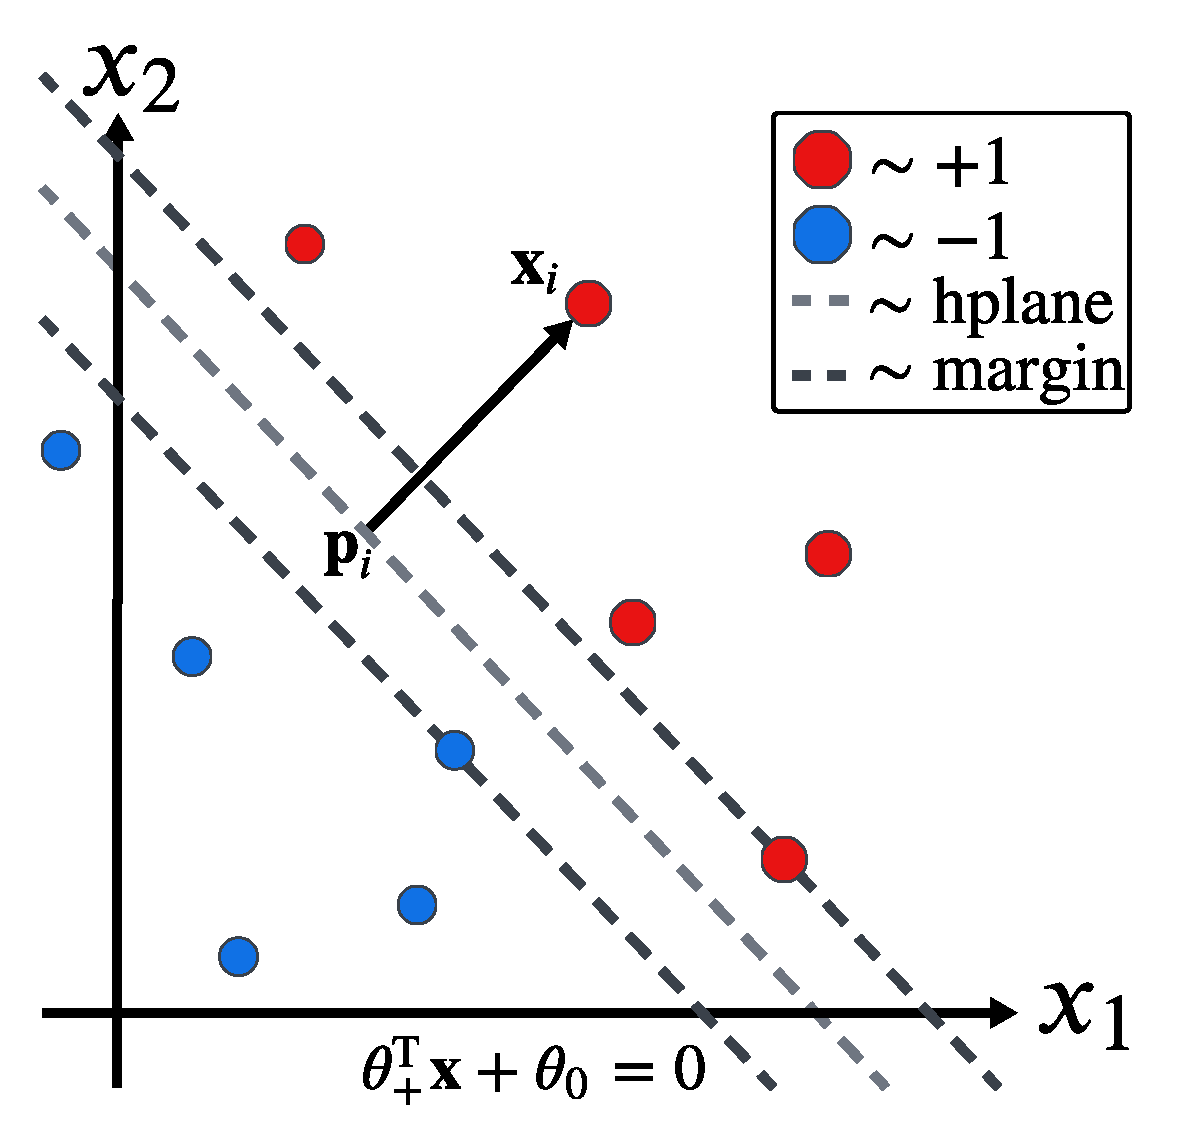
\includegraphics[width=0.75\columnwidth]{./figures/supervised_learning/SVMs/SVM_hard_margin.pdf}
    \caption{A hard-margin SVM in two dimensions.}
    \label{fig:SVM_hard_margin}
\end{figure}

\noindent Let $\mathbf{p}_i$ denote the projection of $\x_i$ onto the hyperplane and let $d_i$ denote the distance between $\mathbf{p}_i$ and $\x_i$. Noting that the normal to the hyperplane is $\theta_+$, we have $\mathbf{p}_i=\x_i-\frac{\theta_+}{||\theta_+||}d_i$ and so
$$
\theta_+^{\text{T}}\l(\x_i-\frac{\theta_+}{||\theta_+||}d_i\r)+\theta_0
=
0
$$
which, after some rearranging, yields
$$
d_i
=
\frac{\theta_+^{\text{T}}\x_i+\theta_0}{||\theta_+||}.
$$
Taking a point $\x_i$ whose class is $-1$ yields $d_i=-\frac{\theta_+^{\text{T}}\x_i+\theta_0}{||\theta_+||}$ and so a neater way of writing this distance for an arbitrary sample $\x_i$ is $d_i=\frac{z_i(\theta_+^{\text{T}}\x_i+\theta_0)}{||\theta_+||}$. Let $d_{\text{min}}=\min_{i=1,\dots,n}d_i$. The idea behind hard-margin SVMs is only applicable to entirely linearly sparable data and effectively boilds down to finding which parameters maximise $d_{\text{min}}$. That is, we look to compute
\begin{align*}
    \thetaOpt
    &=
    \argmax_{(\theta_0,\theta_+)}\l[\min_{i=1,\dots,n}d_i\r]\\
    &=
    \argmax_{(\theta_0,\theta_+)}\l[\min_{i=1,\dots,n}\frac{z_i(\theta_+^{\text{T}}\x_i+\theta_0)}{||\theta_+||}\r]\\
\end{align*}
which we'd like to translate into a convex optimisation problem. First, notice that computing $\thetaOpt$ is equivalent to solving
$$
\max_{(\theta_0,\theta_+)}\frac{r}{||\theta_+||}\text{ s.t. } z_i\l(\theta_+^{\text{T}}\x_i+\theta_0\r)\geq r\text{ } (i=1,\dots,n).
$$
in which $r$ is arbtirarily scalable, so it is equivalent to
$$
\max_{(\theta_0,\theta_+)}\frac{1}{||\theta_+||}\text{ s.t. } z_i\l(\theta_+^{\text{T}}\x_i+\theta_0\r)\geq 1\text{ } (i=1,\dots,n).
$$
This problem is still non-convex so we make a convenient switcheroo in realising that it is equivalent to solving
$$
\min_{(\theta_0,\theta_+)}||\theta_+||^2\text{ s.t. } z_i\l(\theta_+^{\text{T}}\x_i+\theta_0\r)\geq 1\text{ } (i=1,\dots,n)
$$
which is solved in the usual convex problem solving ways.

\subsubsection{Soft-margin SVMs}

Hard-margin SVMs are rarely applicable. In practice, classes are not entirely linearly separable, due to noise and outliers, and so allowing for some misclassification is pragmatic. Going from hard-margin to soft-margin is pretty straightforward, just include some slack variables $\xi=(\xi_1,\dots,\xi_n)$ that ultimately allow the model to violate the constraints while penalising said violations. More precisely, it involves solving
$$
\min_{(\theta_0,\theta_+,\xi)}\l[||\theta_+||^2+\lambda\sum_{i=1}^n\xi_i\r]\text{s.t. } z_i\l(\theta_+^{\text{T}}\x_i+\theta_0\r)\geq 1-\xi_i,\text{ }\xi_i\geq0\text{ } (i=1,\dots,n)
$$
where $\lambda\geq0$ is a regularisation parameter that influences the tradeoff of margin size and misclassification rate. Larger $\lambda$ corresponds to prioritising a larger margin while smaller $\lambda$ corresponds to prioritising the minimisation of misclassification.

\begin{figure}[ht]
    \centering
    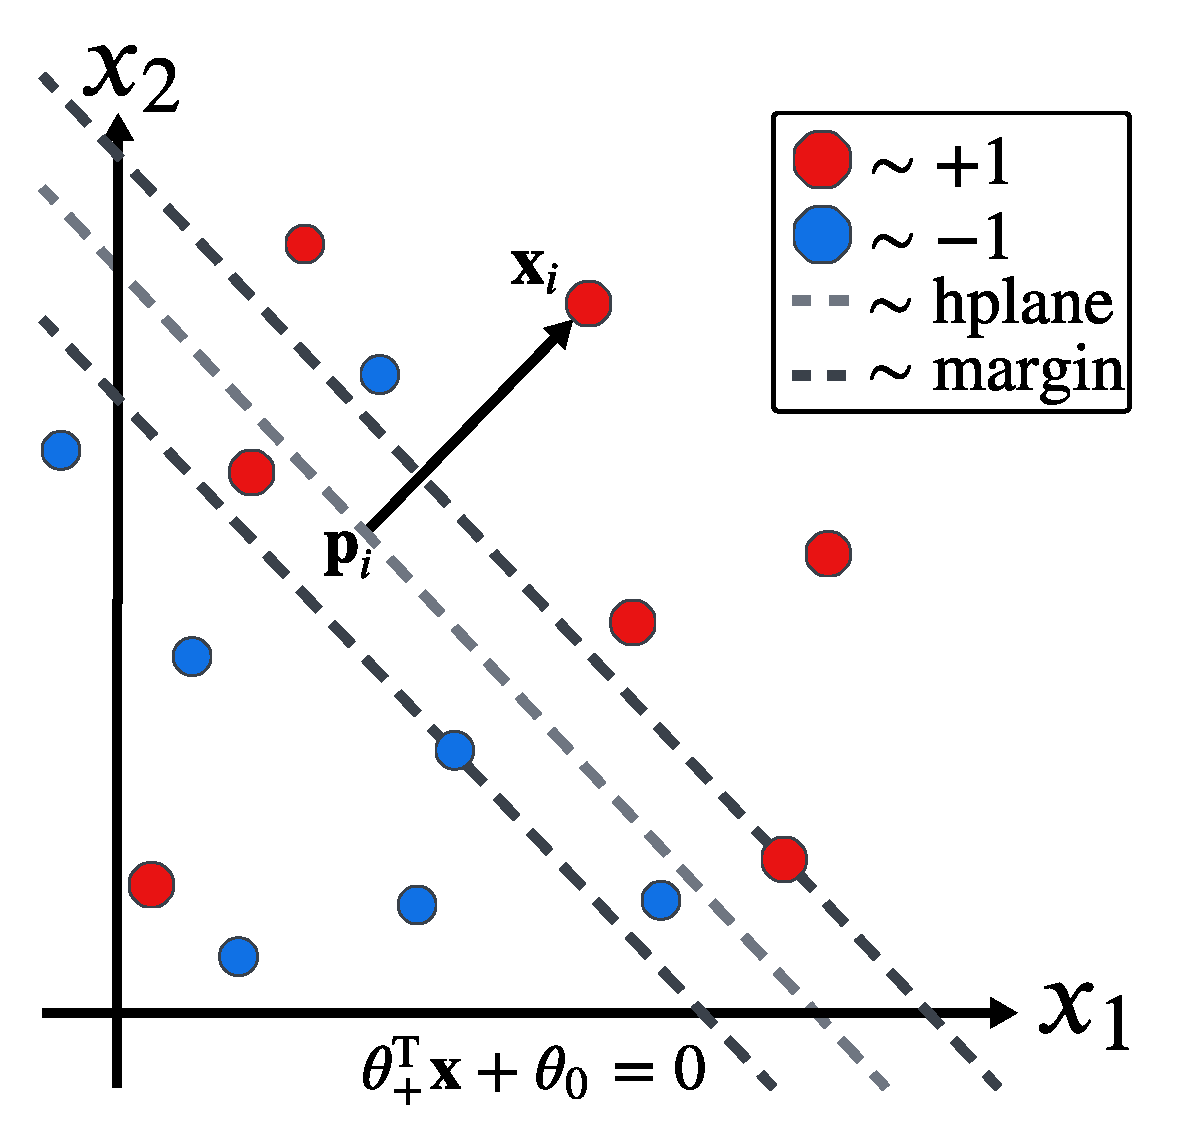
\includegraphics[width=0.75\columnwidth]{./figures/supervised_learning/SVMs/SVM_soft_margin.pdf}
    \caption{A soft-margin SVM in two dimensions. Samples are labelled according to their true class.}
    \label{fig:SVM_soft_margin}
\end{figure}

\noindent As illustrated in \autoref{fig:SVM_soft_margin}, it allows for samples to be closer to the decision boundary than the margin as well as outright misclassifications. Again, it is typically solved in the usual convex problem solving ways. Going a step further, it turns out that this can be simplified to computing
$$
\argmin_{(\theta_0,\theta_+)}\l[||\theta_+||^2+\lambda\sum_{i=1}^n\max\l(0,1-z_i\l(\theta_+^{\text{T}}\x_i+\theta_0\r)\r)\r]
$$
which can be done using gradient descent.

\subsubsection{Non-linear SVMs}
\begin{itemize}
    \item the kernel trick
    \item standard kernels
    \item derivation of standard identity
\end{itemize}
\dots

% decision trees and random forests
\subsection{Decision Trees and Random Forests}
\begin{itemize}
    \item split according to some feature
    \item prune prune prune
\end{itemize}

% handcrafted features
\subsection{Handcrafted Features}
A lost art in the current era :(

% the bias-variance tradeoff
\subsection{The Bias-Variance Tradeoff}
The bias-variance tradeoff is a statement pertaining to how well one can perform supervised learning from datasets. Crudely put, if the model family used to fit is too simple to represent the underlying distributions from which the samples were drawn then our learning method is highly-biased: our method is almost dataset-invariant. Think of fitting a line to a high-degree polynomial. On the other end, if the model family is too complex (e.g. overparameterised) then one might expect to more-easily overfit the underlying distribution. There are too many parameters to twink and tweam so fitting the individal samples is too easy.

\subsubsection{Derivation with MSE loss}
Recall that sample targets pertaining to datasets from which supervised models are learned are effected by noise, i.e. $Y|(X=x)=f(x)+\epsilon(x)$ where $\epsilon(x)\sim\N(0,\sigma^2(x))$ and so
$$
Y|(X=x)
\sim
\N\l(f(x), \sigma^2(x)\r).
$$
We seek to learn an estimate $\hat{f}_{D}$ of $f(x)=\E_Y\l[Y|X=x\r]$ from the dataset $D\subset(\Omega_X\times\Omega_Y)^n$. In other words, the model/estimate $\hat{f}_{D}$ is determined by the realisation $D$ of $\D$ where $\D$ is distributed according to $p(x,y)^{\otimes n}$ for some fixed $n$. As is common in supervised learning contexts, we make use of the expected risk of an estimate $\hat{f}_D$ which is given by
$$
R\l(\hat{f}_D\r)
=
\E_{(X,Y)}\l[\l(Y-\hat{f}_D(X)\r)^2\r]
$$
in which mean square error (MSE) is used as loss. The quantity pertaining to the quality of a learning procedure used to determine $\hat{f}_{D}$ from $D\in\Omega_{\D}$ is given by
\begin{align*}
    \E_{\D}\l[R\l(\hat{f}_{\D}\r)\r]
    &=
    \E_{\D}\l[\E_{(X,Y)}\l[\l(Y-\hat{f}_{\D}(X)\r)^2\r]\r]\nonumber\\
    &=
    \E_{\D}\l[\E_{(X,Y)}\l[\l(Y-f(X)+f(X)-\hat{f}_{\D}(X)\r)^2\r]\r]\nonumber\\
    &=
    \textcolor{c5}{\E_{\D}\l[\E_{(X,Y)}\l[\l(Y-f(X)\r)^2\r]\r]}+
    \textcolor{c11}{\E_{\D}\l[\E_X\l[\l(f(X)-\hat{f}_{\D}(X)\r)^2\r]\r]}\\
    &+\textcolor{c3}{\E_{\D}\l[\E_{(X,Y)}\l[2(Y-f(X))\l(f(X)-\hat{f}_{\D}(X)\r)\r]\r]}.
\end{align*}
Let's address this term-by-term beginning with the term in red. See that
\begin{align*}
    &\hspace{14.52pt}
    \textcolor{c3}{\E_{\D}\l[\E_{(X,Y)}\l[2(Y-f(X))\l(f(X)-\hat{f}_{\D}(X)\r)\r]\r]}\\
    &=
    2\E_{\D}\l[\E_X\l[\E_{Y}\l[(Y-f(X))\l(f(X)-\hat{f}_{\D}(X)\r)|X\r]\r]\r]\\
    &=
    2\E_{\D}\l[\E_X\l[\l(f(X)-\hat{f}_{\D}(X)\r)\E_{Y}\l[Y-f(X)|X\r]\r]\r]\\
    &=
    2\E_{\D}\l[\E_X\l[\l(f(X)-\hat{f}_{\D}(X)\r)\cdot0\r]\r]\\
    &=
    0
\end{align*}
in which the tower property of conditional expectations
\begin{align*}
    \E_{(X,Y)}[g(X,Y)]
    &=
    \iint g(x,y)f_{(X,Y)}(x,y)dxdy\\
    &=
    \int \l(\int g(x,y)f_{Y|X}(y|x)dy\r)f_X(x)dx\\
    &=
    \E_X\l[\E_Y\l[g(X,Y)|X\r]\r]
\end{align*}
is applied. As such, the quantity of interest reduces to only two terms as in
$$
\E_{\D}\l[R\l(\hat{f}_{\D}\r)\r]
=
\textcolor{c5}{\E_{\D}\l[\E_{(X,Y)}\l[\l(Y-f(X)\r)^2\r]\r]}+\textcolor{c11}{\E_{\D}\l[\E_X\l[\l(f(X)-\hat{f}_{\D}(X)\r)^2\r]\r]}
$$
of which we will now address the first in orange. Noting that
$$
\E_{Y}\l[Y-f(x)|X=x\r]
=
0
$$
for all $x\in\Omega_X$ and that what is inside the expectation over $\D$ is independent of $\D$, we see that the first term reduces to
\begin{align*}
    \textcolor{c5}{\E_{\D}\l[\E_{(X,Y)}\l[(Y-f(X))^2\r]\r]}
    &=
    \E_{(X,Y)}\l[(Y-f(X))^2\r]\\
    &=
    \E_X\l[\E_Y\l[(Y-f(X))^2|X\r]\r]\\
    &=
    \E_X\l[\E_Y\l[\l(Y-\E_Y[Y|X]\r)^2|X\r]\r]\\
    &=
    \E_X\l[\text{Var}_Y\l(Y|X\r)\r]\\
    &=
    \E_X[\sigma^2(X)]
\end{align*}
This is simply the expected noise, e.g. due to imperfect calibration in the instruments used to obtain samples, and is typically taken to be constant. Usually, as a constant, it is simply denoted by $\sigma^2$.

For the term in green, let $\bar{f}(x)=\E_{\D}\l[\hat{f}_{\D}(x)\r]$ for all $x\in\Omega_X$ and see that
\begin{align*}
    &\hspace{14.52pt}
    \textcolor{c11}{\E_{\D}\l[\E_X\l[\l(f(X)-\hat{f}_{\D}(X)\r)^2\r]\r]}\\
    &=
    \E_{\D}\l[\E_X\l[\l(f(X)-\bar{f}(X)+\bar{f}(X)-\hat{f}_{\D}(X)\r)^2\r]\r]\\
    &=
    \E_X\l[\l(f(X)-\bar{f}(X)\r)^2\r]+\E_{\D}\l[\E_X\l[\l(\bar{f}(X)-\hat{f}_{\D}(X)\r)^2\r]\r]\\
    &+
    2\E_{\D}\l[\E_X\l[\l(f(X)-\bar{f}(X)\r)\l(\bar{f}(X)-\hat{f}_{\D}(X)\r)\r]\r].
\end{align*}
See that the final term vanishes as $\E_{\D}\l[\bar{f(X)}-\hat{f}_{\D}(X)\r]=0$ and so
\begin{align*}
    &\hspace{14.52pt}
    \textcolor{c11}{\E_{\D}\l[\E_X\l[\l(f(X)-\hat{f}_{\D}(X)\r)^2\r]\r]}\\
    &=
    \E_X\l[\l(f(X)-\bar{f}(X)\r)^2\r]+\E_{\D}\l[\E_X\l[\l(\bar{f}(X)-\hat{f}_{\D}(X)\r)^2\r]\r]\\
    &=
    \E_X\l[\l(f(X)-\bar{f}(X)\r)^2+\E_{\D}\l[\l(\bar{f}(X)-\hat{f}_{\D}(X)\r)^2\r]\r]\\
    &=
    \E_X\l[\l(f(X)-\E_{\D}\l[\hat{f}_{\D}(X)\r]\r)^2+\E_{\D}\l[\l(\hat{f}_{\D}(X)-\E_{\D}\l[\hat{f}_{\D}(X)\r]\r)^2\r]\r].
\end{align*}
Put together, we obtain
\begin{align*}
    &\hspace{14.52pt}
    \E_{\D}\l[R\l(\hat{f}_{\D}\r)\r]\\
    &=
    \E_X\l[\underbrace{\l(f(X)-\E_{\D}\l[\hat{f}_{\D}(X)\r]\r)^2}_{\text{square of bias of estimator}}+\underbrace{\E_{\D}\l[\l(\hat{f}_{\D}(X)-\E_{\D}\l[\hat{f}_{\D}(X)\r]\r)^2\r]}_{\text{variance of estimator}}\r]+\underbrace{\sigma^2}_{\text{noise}}
\end{align*}
where $\sigma^2=\E_X\l[\sigma^2(X)\r]$ (ignore the poor choice of notation). We can crudely summarise it as the sum of the weighted average, according to $p(x)$, of the square of the bias of the learning method, the variance of the estimate according to the dataset from which it is determined and irreducible noise. The irreducible noise is invariant to the learning method and so it's usually ignored in discussions surrounding the bias-variance tradeoff.

\begin{figure}[ht]
    \centering
    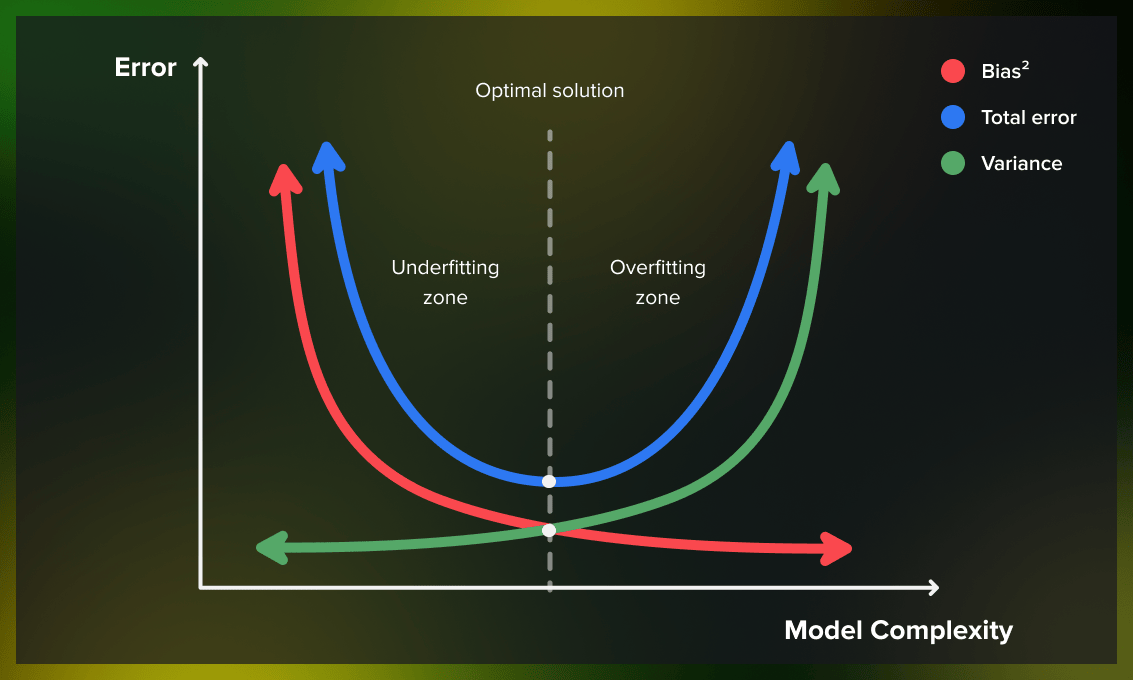
\includegraphics[width=\columnwidth]{./figures/supervised_learning/bias_variance.png}
    \caption{The graph of learning method error against model complexity in terms of bias and variance.}
    \label{fig:bias_variance}
\end{figure}

In brief, if the learned estimate varies a lot as we vary the dataset from which it is determined then the learning method has high variance. This is often due to the estimates in question overfitting the dataset on which they were learned which itself is often due to overparameterisation. If the number of parameters of a model is far higher than is needed then one can easily fit the individal samples from the dataset used during learning. Think of fitting a high degree polynomial to a line. The dataset will consist of points which roughly form a line but the high degree polynomial, if not regularised, can easily fit the samples present in the dataset used to learn (and in doing so fits the noise) resulting in an overfit model.

The flip side of this is an underparameterised model. Since such a model has little hope of fitting the dataset from which it is learned, you'd expect it to rarely overfit (it can't) and to instead be almost invariant to the dataset. That is, no matter which dataset you gave it to learn from, you get a similar model each time. In other words, the learning method (the method of going from dataset to model) is biased. Think of fitting a line to high degree polynomial — no matter what dataset you use, the best fit line will likely not change too much (which is usually a good thing) but the fit itself will never be anything but linear, i.e. always a bad fit. 

With this in mind, when considering which learning method (i.e. model family) to consider when tackling a problem, thought should be given to how complex (i.e. parameter number) the model family should be. Too simple (i.e. too few parameters) and you underfit (high bias, low variance). Too complex (i.e. too many parameters) and you overfit (low bias, high variance). This is nicely illustrated in \autoref{fig:bias_variance} in which we see that there exists a sweet spot in model complexity. A spot in which said model complexity yields some square of bias and some variance but the minimum some of said quantities, i.e. the lowest learning method error. You can think of this plot as the graph of
$$
\l(N\l(\mathcal{A}\r),\E_X\l[R\l(\hat{f}_{\D}(X)\r)\r]\r)
$$
where $N(\mathcal{A})$ denotes the number of parameters of models given by $\mathcal{A}$.

\subsubsection{\textcolor{red}{TODO:} How it motivates regularisation}
For ordinary least squares (OLS), methods of regularisation, such as L1 and L2, introduce some bias but reduce variance. The result is better performance according to MSE.

For classification, as the quantity of data increases, the variance of learned models decreases. As such, if we get more and more data, it might be more tempting to use methods which knowingly have minimal bias as the variance will be taken care of by increased amounts of data. On the other hand, if you have few samples then perhaps consider methods with knowingly little variance, e.g. Bayesian methods.

\subsubsection{Beyond MSE}
Natural question: MSE is a common choice of loss when dealing with regression but not classification, in which cross-entropies are used for loss, so why does every derivation of the bias-variance tradeoff only use MSE? The quick answer is that it's the only choice which yields a relatively simple derivation of this nice decomposition of learning method error into two orthogonal characteristics of the learning method: bias and variance. It turns out that if you instead consider specifically probabilistic classification methods then using expected cross-entropy as loss yields a decomposition into bias and variance but with a different form.

\subsubsection{Double descent}
Double descent refers to a behaviour in which overparameterised models ignore fly in the face of the bias-variance tradeoff. As the number of parameters (i.e. the model complexity) increases beyond a certain point the test error begins to drop. What makes this a phenomenon is that it seems that this threshold is the number of samples used to determine the model. This is illustrated nicely in \autoref{fig:double_descent}.

\begin{figure}[ht]
    \centering
    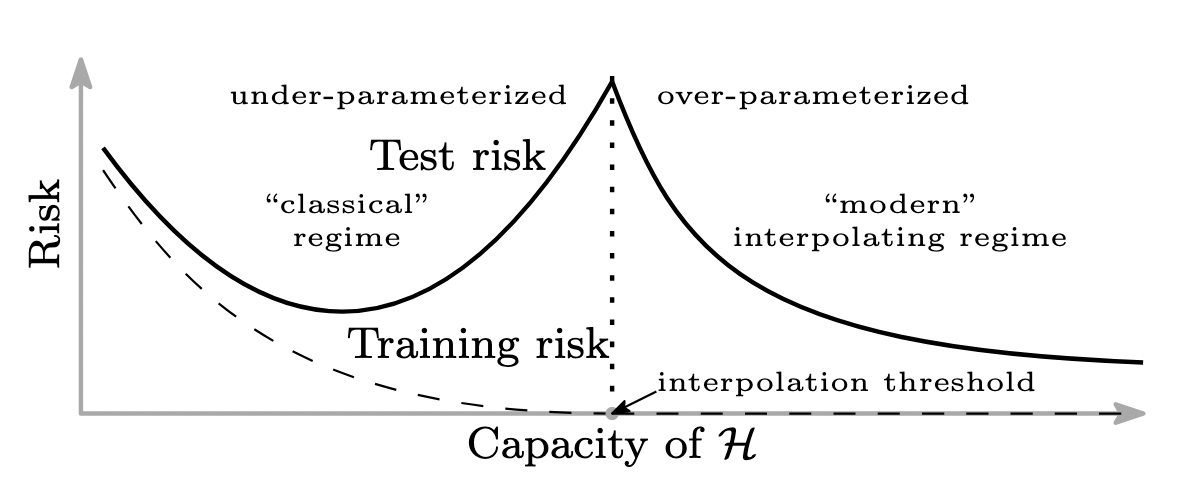
\includegraphics[width=\columnwidth]{./figures/supervised_learning/double_descent.png}
    \caption{\dots}
    \label{fig:double_descent}
\end{figure}

A consequence of this is that very deep neural networks learned using gradient descent do exceptionally well. It flies in the face of conventional wisdom. I'm unaware of anyone that this doesn't surprise. It isn't well-understood. It's related to grokking.

% misc. questions
\addtocontents{toc}{\protect\setcounter{tocdepth}{1}}
\subsection{Misc. questions}
\addtocontents{toc}{\protect\setcounter{tocdepth}{2}}

Some questions to challenge one's understanding.

\begin{tcolorbox}[colback=c2]
\begin{center}
    \textbf{Q1: What are the benefits of using logistic regression over more sophisticated methods?}
\end{center}
\vspace{-8pt}
\begin{itemize}[label=\scriptsize\textbullet,left=0pt]
    \item Its implementation and interpretation are straightforward
    \item If offers a notion of classification confidence which is useful
    \item Statistical tests can be conducted on parameters, e.g. statistical significance tests
\end{itemize}
\end{tcolorbox}

\begin{tcolorbox}[colback=c2]
\begin{center}
    \textbf{Q2: Why not use mean absolute error instead of MSE?}
\end{center}
\vspace{-8pt}
There are many reasons for this, one of which is that often in machine learning and statistics-related contexts one would like to be able to compute the derivative(s) of such a loss function, e.g. in gradient descent, and the presence of an absolute value makes this annoying.

As to why it's useful that the MSE involves the squares of the errors, instead of exponents like $2.05, 3$ or $\pi$, it was best put by this answer to a Stack Exchange answer about the same question\footnote{\url{https://math.stackexchange.com/a/63245}}:

``The variance is the mean squared deviation from the average. The variance of the sum of 10,000 random variables is the sum of their variances. That doesn't work for other powers of the absolute value of the deviation. That means if you roll a die 6,000 times, so that the expected number of 1s you get is 1,000, then you also know that the variance of 1s is $6000\cdot\frac{1}{6}\cdot\frac{5}{6}$ so if you want the probability that the numbner of 1s is between 990 and 1,020, you can approximate the distribution by the normal distribution with the same mean and variance. You couldn't do that if you didn't know the variance, and you couldn't know the variances without additivity of variances, and if the exponent were anything besides 2, then you don't have that. (Oddly, you do have additivity with cubes of the deviations, but not cubes of the absolute values of the deviations)."
\end{tcolorbox}

\begin{tcolorbox}[colback=c2]
\begin{center}
    \textbf{Q3: How can we get an idea of the extent to which our features and output are linearly related without plotting?}
\end{center}
\vspace{-8pt}
To be honest, I thought a streamline test for this existed. As per this Stack Exchange answer\footnote{\url{https://stats.stackexchange.com/a/239142}}, a good method for this is to simply fit a linear and a non-linear model (e.g. a cubic spline smoother model) and see which explains a larger amount of the variance of the output via ANOVA tests.
\end{tcolorbox}

% gradient descent and optimisation techniques
\section{Gradient Descent and its Optimisation}
\dots

% vanilla gradient descent
\subsection{Gradient Descent}
\dots

% momentum
\subsection{Momentum}
\dots

% hyperparam tuning
\subsection{Hyperparameter Tuning}
\dots

% misc. questions
\addtocontents{toc}{\protect\setcounter{tocdepth}{1}}
\subsection{Misc. questions}
\addtocontents{toc}{\protect\setcounter{tocdepth}{2}}

Some questions to challenge one's understanding.

\begin{center}
    \textbf{\textcolor{blue}{Q1:} Why does $f(\mathbf{x})$ ascend most in the direction of $\nabla f(\mathbf{x})$?}
\end{center}

\noindent The following is more of a proof \textit{that} $\nabla f(x)$ yields the direction of steepest ascent not an intuition of \textit{why}. That'll come later.

For some reason, it is typically taken for granted that $f(\mathbf{x})$ would both ascend and ascend \textit{most} in the direction of $\nabla f(\mathbf{x})$. I do not consider this obvious at all, so here is an informal physicist-like argument. Note that in this argument, we consider only unit vectors $\mathbf{v}$. This is because we care only about the direction of such vectors, so size does not matter, and an equation later on simplifies quite nicely due to its unit length. 

In gradient descent, we are looking for the unit vector $\mathbf{v}$ such that $f(\mathbf{x})$ increases most in the direction of $\mathbf{v}$, i.e. we are trying to solve the optimisation problem given by
$$\argmax_{||\mathbf{v}||=1}\Big[f(\mathbf{x}+\eta\mathbf{v})-f(\mathbf{x})\Big]$$
where $\eta>0$. Approximating $f(\mathbf{x}+\eta\mathbf{v})$ by its Taylor approximation
$$
\nabla f(\mathbf{x})\cdot\mathbf{v}\approx\frac{f(\mathbf{x}+\eta\mathbf{v})-f(\mathbf{x})}{\eta},
$$
for small $\eta>0$, yields
$$
f(\mathbf{x}+\eta\mathbf{v})-f(\mathbf{x})
\approx
\nabla f(\mathbf{x})\cdot\eta\mathbf{v}
$$
and so the problem translates to finding the unit vector $\mathbf{v}$ that maximises
$$
\nabla f(\mathbf{x})\cdot\eta\mathbf{v}=||\nabla f(\mathbf{x})||\cdot||\eta\mathbf{v}||\cdot\cos(\theta)=\eta||\nabla f(\mathbf{x})||\cdot\cos(\theta)
$$
where $\theta\in[0,\pi)$ denotes the angle between $\nabla f(\mathbf{x})$ and $\mathbf{v}$. This is clearly maximised when $\cos(\theta)=1$, i.e. when $\theta=0$, and $\mathbf{v}$ has the same direction as $\nabla f(\mathbf{x})$. So $\mathbf{v}$ is a unit vector in the direction of $\nabla f(\mathbf{x})$, i.e. $\mathbf{v}=\frac{\nabla f(\mathbf{x})}{||\nabla f(\mathbf{x})||}$. To see that $f$ ascends after being sent in the direction of $\mathbf{v}=\frac{\nabla f(\mathbf{x})}{||\nabla f(\mathbf{x})||}$ from $\mathbf{x}$ by a distance $\eta>0$, note that
$$
f(\mathbf{x}+\eta\mathbf{v})-f(\mathbf{x})
\approx
\nabla f(\mathbf{x})\cdot\eta\mathbf{v}
=
\eta\frac{\nabla f(\mathbf{x})\cdot\nabla f(\mathbf{x})}{||\nabla f(\mathbf{x})||}
=
\eta||\nabla f(\mathbf{x})||
>
0.
$$
The edge case where $\nabla f(\mathbf{x})=0$ of course corresponds to $f(\mathbf{x})$ being a local maximum.

\vspace{10pt}

\noindent\textbf{Note}: This argument, which utilises a Taylor approximation, relies on a sufficiently small $\eta>0$. Otherwise, the terms in the Taylor approximation of $f(\mathbf{x}+\eta\mathbf{v})$ beyond $\nabla f(\mathbf{x})\cdot\eta\mathbf{v}$ are not necessarily negligible.

\begin{center}
    \textbf{\textcolor{blue}{Q2:} Which loss function is appropriate?}
\end{center}

\noindent Note that these depend on having uniform diversity of classes. If not then use weighted cross-entropy loss functions. There are a ton of machine learning-related scenarios that would need a specially-chosen loss function but the list below is a fine start.

\begin{table}[ht]
    \begin{center}
        \begin{tabular}{c||c}
            \textbf{Task} & \textbf{Loss function}\\
            \hline
            \hline
            Binary classification & Binary cross-entropy\\
            Multi-class classification & Categorical cross-entropy\\
            Regression & Mean square error\\
            Multi-label classification & Binary cross-entropy over each label\\
            \hline
        \end{tabular}
    \end{center}
    \vspace{-15pt}
    \caption{Loss function choices.}
    \label{tab:loss_func_choices}
\end{table}
\noindent Most of these are principled in that their minimisation corrsponds to maximum likelihood estimation.

\begin{center}
    \textbf{\textcolor{blue}{Q3:} How should we choose the learning rate $\eta$?}
\end{center}
This is entirely problem-dependent but $\eta=0.1$ is a great staple choice. If convergence is unstable then try $\eta=0.01$. Other than this line of thinking, there are some `rules of thumb' relating batch number/size to learning rate, otherwise it's a `whatever seems to work best' kind of thing.

\begin{center}
    \textbf{\textcolor{blue}{Q4:} How should we initialise the parameters?}
\end{center}
Xavier initialisation is often-used for neural networks. Maybe things have changed in this regard though; things move fast. Unsure about older architectures.

% neural nets
\section{Neural Networks}
It's often the case that someone's intended meaning when stating `neural networks' is more precisely multi-layer perceptrons (MLPs), perhaps the simplest kind of neural network. Rigorously formulating MLPs is one of those things that's useful to do at least once. Formulating more sophisticated architectures, like CNNs, RNNs, etc., can be done in a much less rigorous manner if your use-case is solving tasks in an engineery way.\\

\noindent\textbf{Note:} Throughout, the terms `neuron' and `node' are synonymous. I use both without realising it at the time of writing.

% neural networks
\subsection{Multi-Layer Perceptrons (MLPs)}

Multi-layer perceptrons (MLPs) are fully-connected feed-forward networks consisting of an input layer (where data is input), hidden layers and an output layer. An MLP with three hidden layers is illustrated in \autoref{fig:MLP}. Each layer is made up of a number of neurons, each of which has a real-valued activation value.  For any node in a non-input layer, its activation value is the output of a non-linear activation function given, as input, the node's real-valued bias plus a weighted sum of the activation values of the neurons in its preceding layer. Regarding their inspiration from the human brain, consider this footnote\footnote{\url{https://stats.stackexchange.com/a/159172}}.

The application of MLPs to learning functions from data is due to their expressivity, expressive-efficiency and tractability. Their expressivity is known due to a proof of their universal function approximation by Cybenko. To add to this, their high expressive-efficiency has been demonstrated empirically and ensures that the number of model components (hidden layers and neurons) needed to represent arbitrary functions is far lower than competing model classes. As for their tractability, MLPs allow for an evaluation of the approximation of the function of interest with complexity quadratic in the number of nodes of each layer of the MLP (after the heavy simplifcation of assuming a roughly equal number of nodes in each layer).

\begin{figure}[ht]
    \centering
    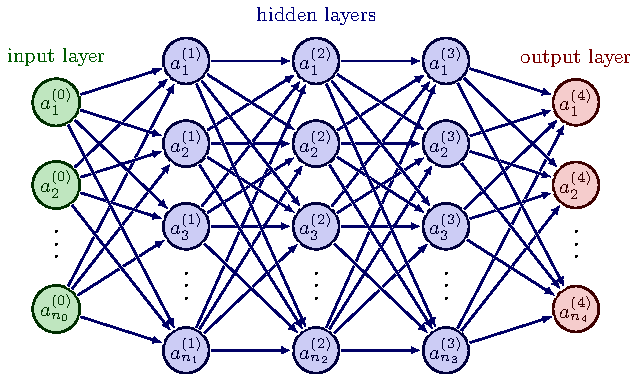
\includegraphics[width=1\linewidth]{./figures/neural_nets/MLP_1.pdf}
    \caption{A multi-layer perceptron (MLP) with $k=3$ hidden layers.}
    \label{fig:MLP}
\end{figure}

For ease of notation, given an MLP with $k$ hidden layers, denote the index of the input layer by $0$, the output layer by $k+1$ and by extension the $j^{\text{th}}$ layer by $j\in\{0,\dots,k+1\}$. Additionally, note the following:
\begin{itemize}
    \item Let $n_j\in\mathbb{Z}_{\geq1}$ denote the number of neurons in layer $j$.
    \item Let $a_i^{(j)}\in\mathbb{R}$ denote the activation value of neuron $i$ in layer $j$.
    \item Let $w_{i,l}^{(j)}\in\mathbb{R}$ denote the weight associated with the edge to neuron $i$ in layer $j\in\{1,\dots,k+1\}$ from neuron $l$ in layer $j-1$.
    \item Let $b_i^{(j)}\in\mathbb{R}$ denote the bias of neuron $i$ in layer $j\in\{1,\dots,k+1\}$.
    \item Let $\sigma_j:\mathbb{R}\rightarrow\mathbb{R}$ denote the non-linear activation function of layer $j\in\{1,\dots,k+1\}$.
\end{itemize}

\noindent From here we can express the activation value of any neuron in a non-input layer in terms of the activation values of the neurons in the layer which precedes it as
\begin{align*}
    a_i^{(j+1)}
    &=
    \sigma_{j+1}\l(
    \sum_{l=1}^{n_j} w_{i,l}^{(j+1)}a_l^{(j)} + b_i^{(j+1)}
    \r)\\
    &=
    \sigma_{j+1}\l(
    \l[w_{i,1}^{(j+1)} \dots w_{i,n_j}^{(j+1)}\r]
    \begin{bmatrix}
        a_1^{(j)}\\
        \vdots\\
        a_{n_j}^{(j)}
    \end{bmatrix}
    +
    b_i^{(j+1)}
\r)
\end{align*}
for $j\in\{0,\dots,k\}$. The reason for writing the second equality above, involving the dot product of two vectors, is that it helps us to see how using matrix-vector notation allows us to write an elegant and compact expression for the activation values of all nodes in a non-input layer in terms of the activation values of the neurons belonging to its preceding layer as
$$
\begin{bmatrix}
    a_1^{(j+1)}\\
    \vdots\\
    a_{n_{j+1}}^{(j+1)}
\end{bmatrix}
=
\sigma_{j+1}\l(
\begin{bmatrix}
    w_{1,1}^{(j+1)} & \dots & w_{1,n_j}^{(j+1)}\\
    \vdots & \ddots & \vdots\\
    w_{n_{j+1},1}^{(j+1)} & \dots & w_{n_{j+1},n_j}^{(j+1)}
\end{bmatrix}
\begin{bmatrix}
    a_1^{(j)}\\
    \vdots\\
    a_{n_j}^{(j)}
\end{bmatrix}
+
\begin{bmatrix}
    b_1^{(j+1)}\\
    \vdots\\
    b_{n_{j+1}}^{(j+1)}
\end{bmatrix}
\r)
$$
which we abbreviate to
$$
\mathbf{a}^{(j+1)}=\sigma_{j+1}\l(\mathbf{W}^{(j+1)}\mathbf{a}^{(j)}+\mathbf{b}^{(j+1)}\r)
$$
where the activation function $\sigma_{j+1}$ is applied element-wise.

If we fix the structure and choice of activation functions of an MLP then all that is left to learn are its weights and biases. This is often done using gradient descent to minimise some loss function in which gradients are computed via back-propagation. Such a loss function can be a principled measure, e.g. corresponding to maximum likelihood, but this is not always necessary: ad-hoc loss functions are sometimes employed.

\subsubsection{Constructive example: The algebra}

\textcolor{red}{fix this figure}

\begin{figure}[ht]
    \centering
    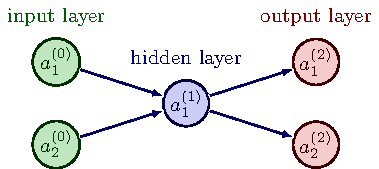
\includegraphics{./figures/neural_nets/MLP_2.pdf}
    \caption{A neural network with $k=1$ hidden layer.}
    \label{fig:neural_nets_simple_example}
\end{figure}

\noindent Consider the neural network in \autoref{fig:neural_nets_simple_example} whose input, hidden and output layers consist of two, one and two neurons respectively. With such a simple neural network, we may explicitly express the output neurons $a_1^{(2)}$ and $a_2^{(2)}$ in terms of the input neurons $a_1^{(0)}$ and $a_2^{(0)}$. We see that $n_0=2$, $n_1=1$ and $n_2=2$ and so
$\mathbf{W}^{(1)}=
\begin{bmatrix}
    w_{1,1}^{(1)} & w_{1,2}^{(1)}
\end{bmatrix}
$
and
$\mathbf{W}^{(2)}=
\begin{bmatrix}
    w_{1,1}^{(2)}\\
    w_{2,1}^{(2)}
\end{bmatrix}.
$
Noting additionally that $\mathbf{b}^{(1)}=b_1^{(1)}$ and
$\mathbf{b}^{(2)}=
\begin{bmatrix}
    b_{1}^{(2)}\\
    b_{2}^{(2)}
\end{bmatrix}$
we can explicitly express the activation of the single neuron in the hidden layer as
\begin{align*}
\mathbf{a}^{(1)}
&=
\sigma_1\l(\mathbf{W}^{(1)}\mathbf{a}^{(0)}+\mathbf{b}^{(1)}\r)\\
&=
\sigma_1\l(w_{1,1}^{(1)}a_1^{(0)}+w_{1,2}^{(1)}a_2^{(0)}+b_1^{(1)}\r)
\end{align*}
which is just the scalar value $a_1^{(1)}$. For the output layer, we have
\begin{align*}
\mathbf{a}^{(2)}
&=
\sigma_2\l(\mathbf{W}^{(2)}\mathbf{a}^{(1)}+\mathbf{b}^{(2)}\r)\\
&=
\sigma_2\l(
\begin{bmatrix}
    w_{1,1}^{(2)}a_1^{(1)} + b_1^{(2)}\\
    w_{2,1}^{(2)}a_1^{(1)} + b_2^{(2)}
\end{bmatrix}
\r)\\
&=
\sigma_2\l(
\begin{bmatrix}
    w_{1,1}^{(2)}\sigma_1\l(w_{1,1}^{(1)}a_1^{(0)}+w_{1,2}^{(1)}a_2^{(0)}+b_1^{(1)}\r) + b_1^{(2)}\\
    w_{2,1}^{(2)}\sigma_1\l(w_{1,1}^{(1)}a_1^{(0)}+w_{1,2}^{(1)}a_2^{(0)}+b_1^{(1)}\r) + b_2^{(2)}
\end{bmatrix}
\r)\\
&=
\begin{bmatrix}
    \sigma_2\l(w_{1,1}^{(2)}\sigma_1\l(w_{1,1}^{(1)}a_1^{(0)}+w_{1,2}^{(1)}a_2^{(0)}+b_1^{(1)}\r) + b_1^{(2)}\r)\\
    \sigma_2\l(w_{2,1}^{(2)}\sigma_1\l(w_{1,1}^{(1)}a_1^{(0)}+w_{1,2}^{(1)}a_2^{(0)}+b_1^{(1)}\r) + b_2^{(2)}\r)
\end{bmatrix}.
\end{align*}

\noindent As such, the activations of the output neurons are given by
\begin{align*}
    a_1^{(2)}&=\sigma_2\l(w_{1,1}^{(2)}\sigma_1\l(w_{1,1}^{(1)}a_1^{(0)}+w_{1,2}^{(1)}a_2^{(0)}+b_1^{(1)}\r) + b_1^{(2)}\r)\\
    a_2^{(2)}&=\sigma_2\l(w_{2,1}^{(2)}\sigma_1\l(w_{1,1}^{(1)}a_1^{(0)}+w_{1,2}^{(1)}a_2^{(0)}+b_1^{(1)}\r) + b_2^{(2)}\r).
\end{align*}

\subsubsection{Constructive example — Subbing values in}

\noindent\textbf{Note}: The weights and biases of a neural network are typically learned during training, i.e. they are parameters to be tweaked and tuned until the corresponding model performs sufficiently well. They are not taken randomly as is done here for the sake of example.\\

\noindent Consider a neural network as in \autoref{fig:neural_nets_simple_example}. For the weights and biases, take
\begin{align*}
    w_{1,1}^{(1)} & =  0.5 & w_{1,1}^{(2)} &= 0.7 \\
    w_{1,2}^{(1)} & = -0.5 & w_{1,2}^{(2)} &= 0.3 \\
    b_1^{(1)}     & =  0.1 & b_1^{(2)}     & =  0.2 \\
                  &        & b_2^{(2)}     & = -0.2
\end{align*}
and for the activation functions $\sigma_1$ and $\sigma_2$ take ReLU, i.e. $\sigma_i(x)=\max(0, x)$.  Finally, take the input neuron values $a_1^{0}=5$ and $a_2^{0}=2$. Explicitly computing the activation values of the output neurons yields
\begin{align*}
    a_1^{(2)}
    &=
    \max(0, 0.7\cdot\max(0, 0.5\cdot5-0.5\cdot2+0.1)+0.2)\\
    &=
    \max(0, 0.7\cdot1.6+0.2)\\
    &=1.32
\end{align*}
and
\begin{align*}
    a_2^{(2)}
    &=
    \max(0, 0.3\cdot\max(0, 0.5\cdot5-0.5\cdot2+0.1)-0.2)\\
    &=
    \max(0, 0.3\cdot1.6-0.2)\\
    &=0.28.
\end{align*}
To confirm these values against the same neural network set up using TensorFlow, consider \texttt{nn\_constructive\_example.py} found \href{https://gitlab.com/dewibatista/master/-/tree/main/_Done/Personal}{here}.

% universal function approximation theorem
\subsubsection{Universal function approximation}
\label{subsubsec:universal_function_approximation_theorem}
Polynomials have one via Wasserstein. But polynomials have low expressive-efficiency. Good motive for MLPs and architectures often-labelled neural networks more generally.

% depth over width
\subsubsection{Depth $>$ Width}
\label{subsubsec:deep_MLPs}
The complexity of a forward pass of an MLP can be expressed in terms of the number of nodes in each layer as
$$
\mathcal{O}
\l(
\sum_{j=0}^{k+1}n_{j-1}\cdot n_j
\r).
$$
Very crudely supposing $n_0=\dots=n_{k+1}=n$ yields a complexity of
$$
\mathcal{O}((k+1)n^2),
$$
i.e. complexity grows linearly in the number of layers and quadratically in the number of neurons per layer. So we argue for increasing depth over width.

A perhaps more important result is from using MLPs for classification. Geomentrically, they do this by splitting some space into a bunch of regions. It turns out that the number of regions by which a single-layer MLP with $n$ neurons in its hidden layer splits the space is bounded above by
$$
\frac{1}{2}(n^2+n+2)
$$
which is quadratic in $n$. For an MLP with $k$ hidden layers of $n$ neurons each, the number of regions by which the space is split is bounded above by
$$
\frac{1}{2}(n^2+n+2)\l(\frac{n}{n_0}+1\r)^{n_0(k-1)}
$$
which is exponential in $k$. Again, we argue for increasing depth $k$ over width $n$.

There's something to be said about the fact that these are upper bounds and to what extent the bounds are tight in practice. Another worthwhile question is: to what extent do contemporary methods of learning the parameters of such architectures make use of this improved number of regions? Do gradient descent-based methods utilise this increase in number of regions perfectly? No, but the study of this sort of thing is worthy of a career so I won't go into more detail about it beyond interesting results, once I come across them.

% backprop
\subsection{Backpropagation for MLPs}
\label{subsec:backprop}

As with formulating MLPs, it's good to rigorously express backpropagation at least once in life, so here it is. It's sort of strange that I haven't done this yet and simply trust that it works while having only an intuitive idea of it up to now (August 2025).

Chain rule/automatic differentiation to learn the parameters from data. Very often it helps us perform numerical maximum likelihood (depends on the loss function invoked).

% convolutional neural networks
\subsection{Convolutional Neural Networks (CNNs)}
\label{subsec:conv_neural_networks}

\textbf{Note:} The terms `kernel' and `filter' are synonymous in this subsection.\\

\noindent Convolutional neural networks (CNNs) are neural networks whose architectures are designed to process image data. Illustrated in \autoref{fig:CNN_frog}, their architecture can be described on a high level as consisting of two parts. The first part performs feature extraction through convolutions and pooling. The second part is an MLP which uses the extracted feature values to produce the overall model's output, e.g. the probability that the input object belongs to a given class. Feature extraction into MLP, pretty intuitive.

\begin{figure}[ht]
    \centering
    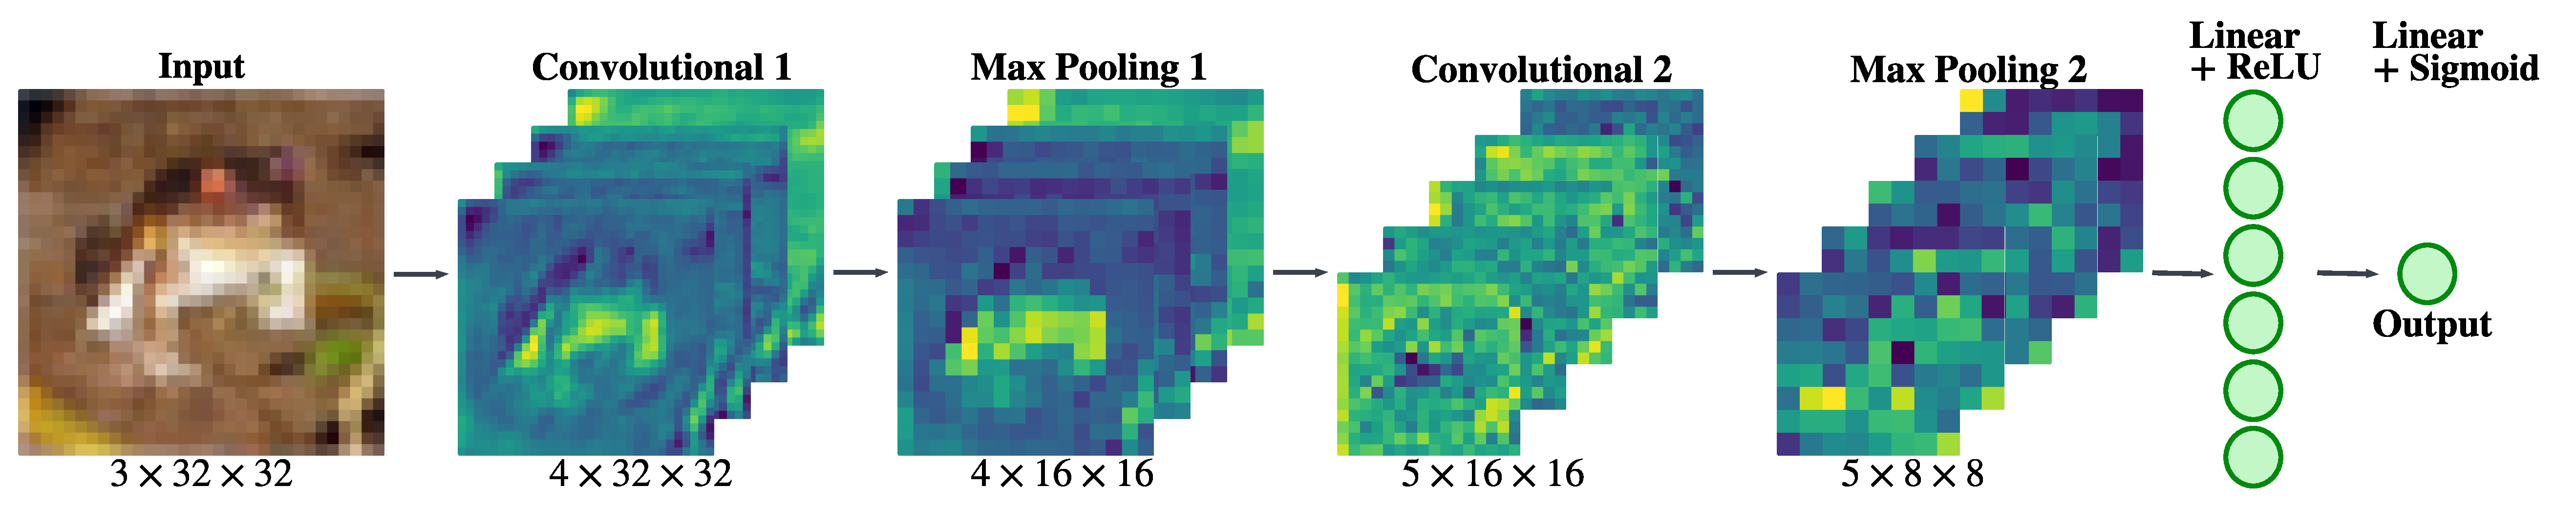
\includegraphics[width=1\textwidth]{./figures/neural_nets/CNN_frog.pdf}
    \caption{A binary classification CNN processing an image of a frog.}
    \label{fig:CNN_frog}
\end{figure}

Before these deep learning architectures, researchers would have use handcrafted features and feed the feature values to a given model, e.g. an SVM for classification. Humans turn out to be far worse at knowing what features to use than well-trained machine learning models. So how do these earlier layers in CNN architectures perform feature extraction? Convolution and pooling layers.

\subsubsection{Convolutions}
Convolution operations involve using a square matrix to, in some sense, summarise the information embedded in the parts of the imaage which it traverses over. This square matrix is referred to as a filter. It's sometimes referred to as a kernel and I tend to unconsciously switch which I use. You can think of this convolution operation as a sort of dot product between the filter and the grid of pixel values it is on top of at that point.

More formally, given a feature map $I\in\mathbb{R}^{C\times W\times H}$ and a kernel $K\in\mathbb{R}^{C\times k\times k}$ with $k<W$ and $k<H$, the feature map $F=K*I\in\mathbb{R}^{W'\times H'}$ given by the convolution of $K$ over $I$ is given by
$$
F_{i,j}
=
\sum_{c=1}^C\sum_{x=1}^{k}\sum_{y=1}^{k}K_{c,x,y}\cdot I_{c,i+x,i+y}+b_c
$$
where $b_c$ is the kernel's bias in channel $c$. Note that this notation is intended to illustrate what a convolution looks like algebraically. As it stands, what's written above does not account for padding, stride, etc. For a simpler illustration, consider \autoref{fig:convolution_operation}.

\begin{figure}[ht]
    \centering
    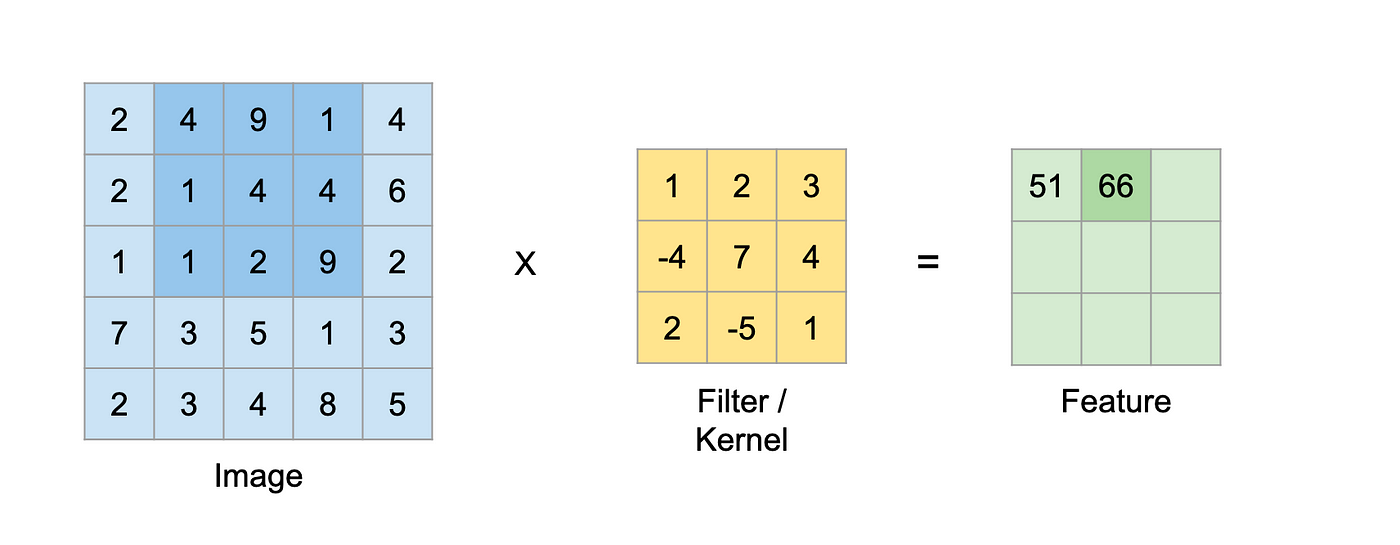
\includegraphics[width=1\textwidth]{./figures/neural_nets/CNN_convolution.png}
    \caption{Convolution without bias.}
    \label{fig:convolution_operation}
\end{figure}

Generally, earlier convolutions in a CNN architecture extract higher level features, like edges and textures, while later convolutions extract lower level features which are not human-interpretable. This is observed in \autoref{fig:CNN_frog} where after the first convolutional layer one can still see a resemblance of the input image of a frog. The feature maps produced by the second convolutional layer do not maintain a human-interpretable resemblance of the frog.

\subsubsection{Pooling}
Pooling operations reduce the spatial dimensions of a given feature map by, in some sense, clustering certain parts of the feature map. There's not much point to writing this mathematically rigorously. Instead, consider \autoref{fig:pooling}. Pooling has a ton of flavours: max, min, average and more.

\begin{figure}[ht]
    \centering
    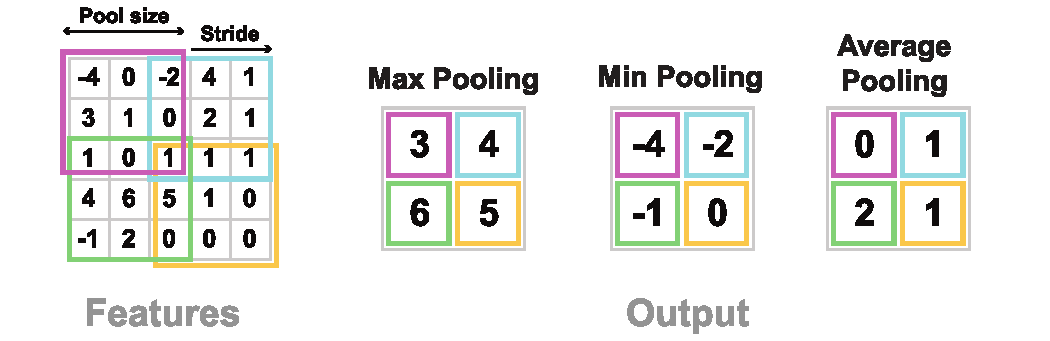
\includegraphics[width=1\textwidth]{./figures/neural_nets/CNN_pooling.pdf}
    \caption{The core flavours of pooling.}
    \label{fig:pooling}
\end{figure}

\noindent I typically just pick max pooling and see how it does. A nice benefit of pooling is improved translation-invariance. Ideally, our model would classify an image in a similar enough way to how it'd classify the same image but slightly shifted. What is meant here is very problem-dependent so take it with a grain of salt. Hopefully the idea is clear anyway. Another benefit to pooling the reduced compute.

\subsubsection*{Output dimensions of convolutions and pooling}
Given a feature map $F\in\mathbb{R}^{W\times H}$, suppose we compute the convolution $O\in\mathbb{R}^{W'\times H'}$ of the kernel $K\in\mathbb{R}^{k\times k}$ over $F$ with uniform padding $P$ and stride $S$. The precise dimensions $W'$ and $H'$ of the new feature map $O$ are given by
$$
W'
=
\l\lfloor
\frac{W+2P-k}{S}
\right\rfloor
+1
$$
and
$$
H'
=
\l\lfloor
\frac{H+2P-k}{S}
\right\rfloor
+1.
$$
It's not too tricky to derive these. It's the kinda thing you do once and never again.

\subsubsection{Backpropagation for CNNs}
We've already seen how to backprop through the MLP component. We haven't seen how to backprop through convoluationa/pooling layers yet. Ultimately, similar idea as for MLPs: automatic differentiation, chain rule, bla bla bla\footnote{\url{https://www.quarkml.com/2023/07/backward-pass-in-convolutional-neural-network-explained.html}}.

% recurrent neural networks
\subsection{Recurrent Neural Networks (RNNs)}
\dots

\subsubsection{Long Short-Term Memory (LSTMs)}
\dots

\subsubsection{Gated Recurrent Units (GRUs)}
\dots

% autoencoders
\subsection{Autoencoders}
\label{sec:autoencoders}
An autoencoder $(\Omega_{\X},d,\theta,\phi)$ consists of a sample space $\Omega_{\X}\subset\mathbb{R}^n$, a latent dimension $d\in\mathbb{Z}_{\geq1}$, an encoder $\theta:\mathbb{R}^n\to\mathbb{R}^d$ and a decoder $\phi:\mathbb{R}^d\to\mathbb{R}^n$. Using a subset of $\Omega_{\X}$, one typically learns the encoder $\theta$ and the decoder $\phi$ with the goal of approximating the identity on $\Omega_{\X}$ via $\phi\circ \theta$. That is, roughly put, one seeks to obtain an encoder/decoder pair such that $\phi(\theta(\x))\approx\x$ for all $\x\in\Omega_{\X}$.

\begin{figure}[ht]
    \centering
    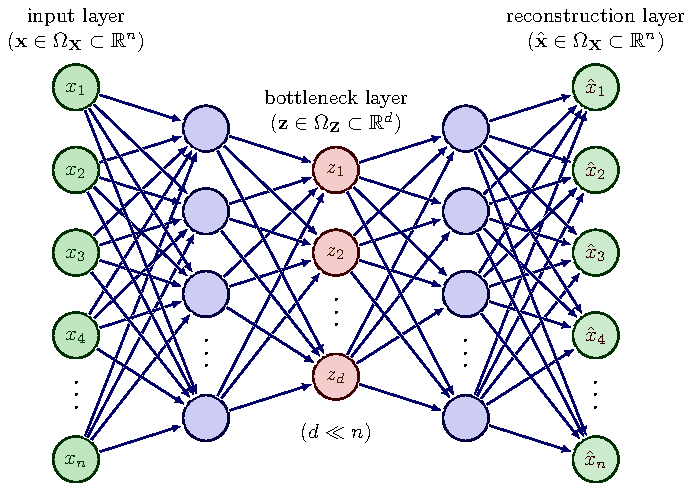
\includegraphics{./figures/neural_nets/AE_autoencoder.pdf}
    \caption{An autoencoder in which $\theta$ and $\phi$ are fit using multi-layer perceptrons (MLPs).}
    \label{fig:autoencoder}
\end{figure}

In intuitive terms, one can see the encoder $\theta$ as a compressor of samples in $\Omega_{\X}$ to their compressed (or latent) representation in $\mathbb{R}^d$ and so one might refer to the image of $\theta$ as the latent space $\Omega_{\Z}$. Similarly, the decoder $\phi$ can be seen as a decompressor of compressed representations $\z\in\Omega_{\Z}$ yielding the original sample $\x$. In line with this notion of an autoencoder as a compressor/decompressor, the latent dimension $d$ is typically taken to be far smaller than the dimension of the distribution of interest, i.e. $d\ll n$. Of course, when $d\ll n$, learning such mappings $\theta$ and $\phi$ typically involves some loss of information if $\Omega_{\X}$ is a manifold whose intrinsic dimension is greater than $d$. That is, autoencoders are typically lossy compressors.

\begin{example}
    Suppose $\Omega_{\X}=\{(a,a,b)\in\mathbb{R}^3:||(a,a,b)||\leq1\}$ and $d=2$. One immediately notices that $\Omega_{\X}$ is a two-dimensional surface embedded in $\mathbb{R}^3$ as it is the intersection of the unit ball and the plane $\{(a,a,b):a,b\in\mathbb{R}\}$. To produce representations of $\x=(a,a,b)\in\Omega_{\X}$ in $\mathbb{R}^2$ (i.e. to compress a sample) one might employ the encoder $\theta_2(x,y,z)=(x,z)$. To reconstruct samples from their latent representation (i.e. to decompress) one might employ the decoder $\phi_2(x,z)=(x,x,z)$. The autoencoder $(\Omega_{\X},2,\theta_2,\phi_2)$ offers lossless compression on the sample space of interest as $(\phi_2\circ\theta_2)(\x)=\x$ for all $\x\in\Omega_{\X}$.

    If we instead desire latent representations of $\x=(a,a,b)\in\Omega_{\X}$ in $\mathbb{R}$, i.e. if $d=1$, one might employ the encoder $\theta_1(x,y,z)=x$ and the decoder $\phi_1(x)=(x,x,x)$. The autoencoder $(\Omega_{\X},1,\theta_1,\phi_1)$ offers lossy compression, i.e. some information pertaining to a sample is lost in compressing and then decompressing it as $(\phi_1\circ\theta_1)(a,a,b)=(a,a,a)$ for all $a,b\in\mathbb{R}$.
\end{example}

One's tolerance for the loss incurred by a given encoder/decoder pair is task-dependent. Given a dataset $\mathcal{D}=\{\x_1,\dots,\x_M\}\subset\Omega_{\X}$ and a latent dimension $d$, one might compute the pair $(\theta^*,\phi^*)\in\Theta\times\Phi$ which minimises the empirical risk over $\mathcal{D}$ where $\Theta$ and $\Phi$ are chosen function classes. That is, computing
$$
(\theta^*,\phi^*)
=
\argmin_{(\theta,\phi)\in\Theta\times\Phi}
\sum_{i=1}^M||\x_i-\phi(\theta(\x_i))||^2.
$$
If the function classes permit for computing the gradients of $\theta\in\Theta$ and $\phi\in\Phi$ then this computation may be done using gradient descent. For example, one could take $\Theta$ and $\Phi$ to be the classes of MLPs of appropriate input and output dimensions, as illustrated in \autoref{fig:autoencoder}.

% skip connections
\addtocontents{toc}{\protect\setcounter{tocdepth}{1}}
\subsection{Skip Connections/Residual Networks}
\addtocontents{toc}{\protect\setcounter{tocdepth}{2}}
\begin{itemize}
    \item Most intuitive benefit: it helps prevent some layer in the architecture from degrading the input entirely. It's like a nice reminder to the model what it was working from before it got to this point
    \item Reduces vanishing or exploding gradients: opens the door to far deeper architectures
    \item Ensures that the model has to learn the residual as opposed to the full underlying function: faster convergence usually
    \item Takes pressure off parameter initialisation: if you set parameters to zero then initially model is just the identity and learning from there is feasible
\end{itemize}

% misc. questions
\addtocontents{toc}{\protect\setcounter{tocdepth}{1}}
\subsection{Misc. questions}
\addtocontents{toc}{\protect\setcounter{tocdepth}{2}}

Some questions to challenge one's understanding.

\begin{center}
    \textbf{\textcolor{blue}{Q1:} How does one prevent overfitting in NNs?}
\end{center}
\textbf{1) Early stopping:} Split training into training and validation sets. After each epoch (or every few), compute both training and validation losses. If training loss is decreasing while validation loss is not decreasing then you're at risk of overfitting. For illustration, consider \autoref{fig:early_stopping} in which the training loss continues to decrease in the number of epochs while the validation loss seems to reach its lowest value around epoch 28.

\begin{figure}
    \centering
    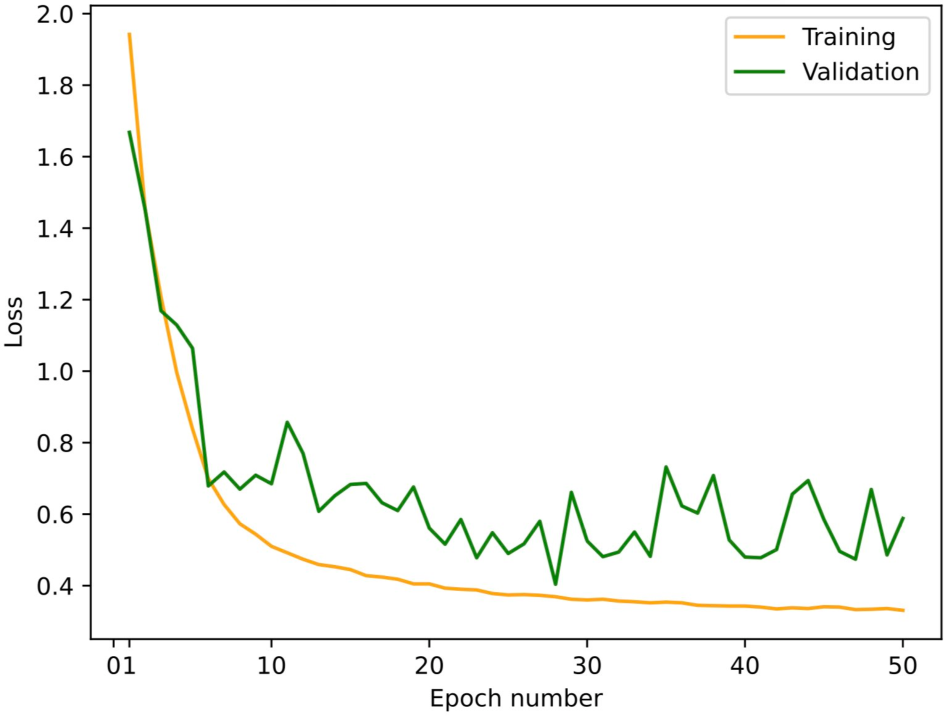
\includegraphics[width=0.75\textwidth]{./figures/neural_nets/REG_early_stopping.pdf}
    \caption{Training and validation losses over 50 epochs for some model.}
    \label{fig:early_stopping}
\end{figure}

\noindent If you observe this for sufficiently many consecutive epochs then you can stop training and use the parameters pertaining to the epoch at which the validation loss was lowest. To do this, at each epoch during training, save the parameters of the current epoch if they offer a lower validation loss than at any epoch before. This is often referred to as a checkpoint within the training process and the parameters are saved in a \texttt{.ckpt} file.\\

\noindent\textbf{2) Dropout:} We don't want to be overly-reliant on any given subset of neurons. To prevent such dependencies, at each epoch, independently set the activation of each neuron to 0 with probability $p$. This way some portion of neurons are silenced during the training epoch. As a result, its corresponding parameters (weights and bias) are not updated during backpropagation — it is truly silenced. This idea is illustrated in \autoref{fig:dropout}. Do not perform dropout when testing.

\begin{figure}[ht]
    \centering
    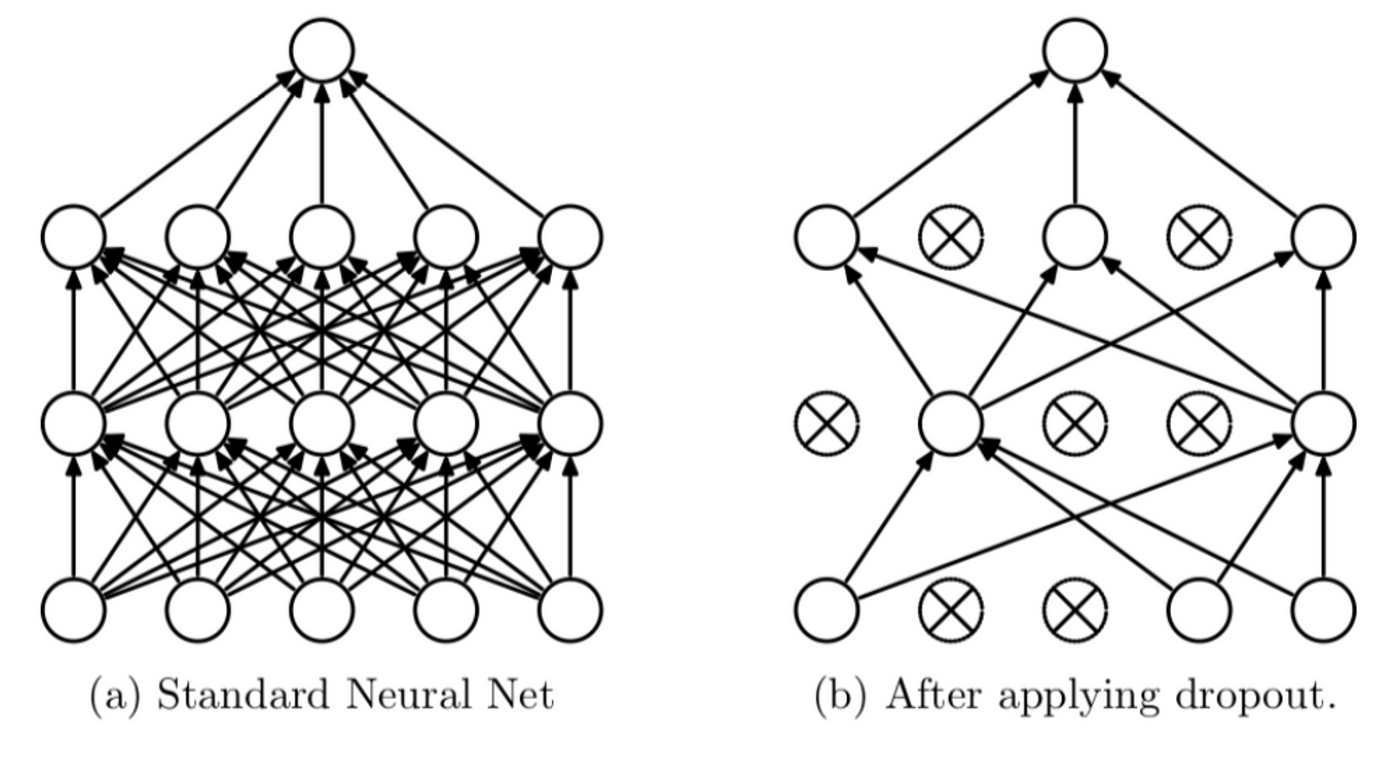
\includegraphics[width=0.75\textwidth]{./figures/neural_nets/REG_dropout.png}
    \caption{Dropout to prevent overdependence on given neurons.}
    \label{fig:dropout}
\end{figure}

\begin{center}
    \textbf{\textcolor{blue}{Q2:} What is the purpose of activation functions?}
\end{center}
Without the application of at least one activation function, the values of the output neurons would simply be the result of matrix-vector multiplication and vector addition. That is to say, the output of the neural network, without an any activation function, would be a purely linear transformation of the input. The issue with this is that most problems require some degree of non-linearity. The staple example of this is the classification of two-dimensional samples which are not linearly-separable. Two such cases are illustrated in \autoref{fig:non_linearly_separable}.

\begin{figure}[ht]
    \centering
    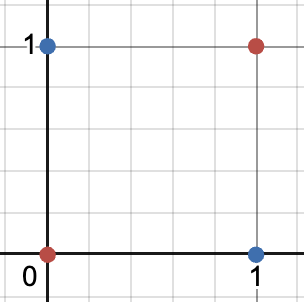
\includegraphics[width=0.40\columnwidth]{./figures/neural_nets/NLA_xor.png}
    \hspace{20pt}
    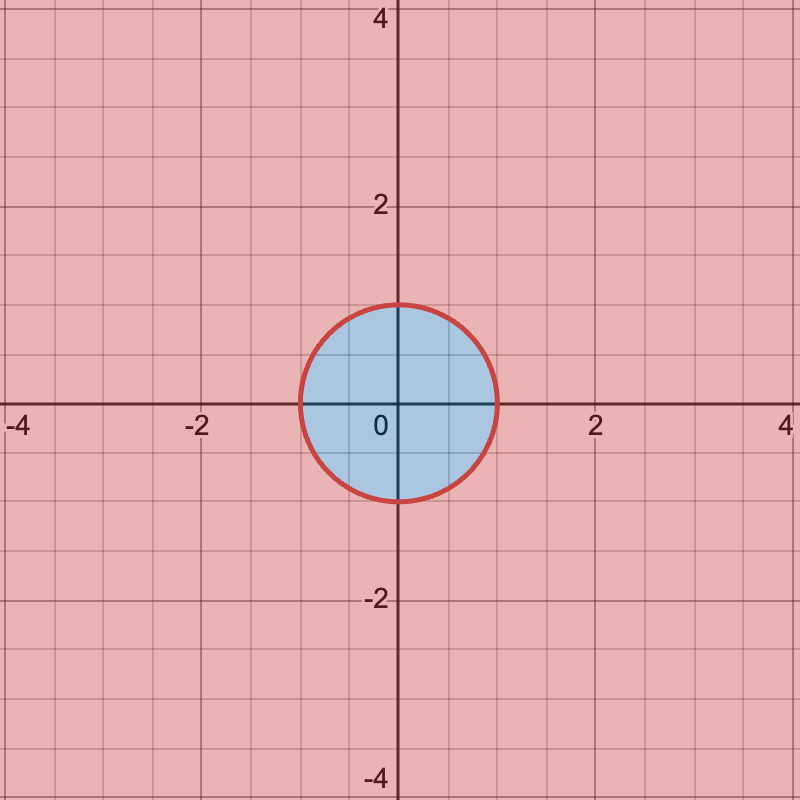
\includegraphics[width=0.40\columnwidth]{./figures/neural_nets/NLA_circle.png}
    \caption{Examples of samples belonging to classes that are not linearly-separable.}
    \label{fig:non_linearly_separable}
\end{figure}

The point is that there is no line that would separate the classes in either case: non-linearity is needed! In the latter case, it is desirable to be able to somehow punch the interior of the unit disc to form a blue mountain with the surrounding ground covered in red. This can be achieved by the non-linear transformation $\phi(x,y)=\max(0,1-(x^2+y^2))$ which is illustrated in \autoref{fig:non_lin_transformation}.

\begin{figure}[ht]
    \centering
    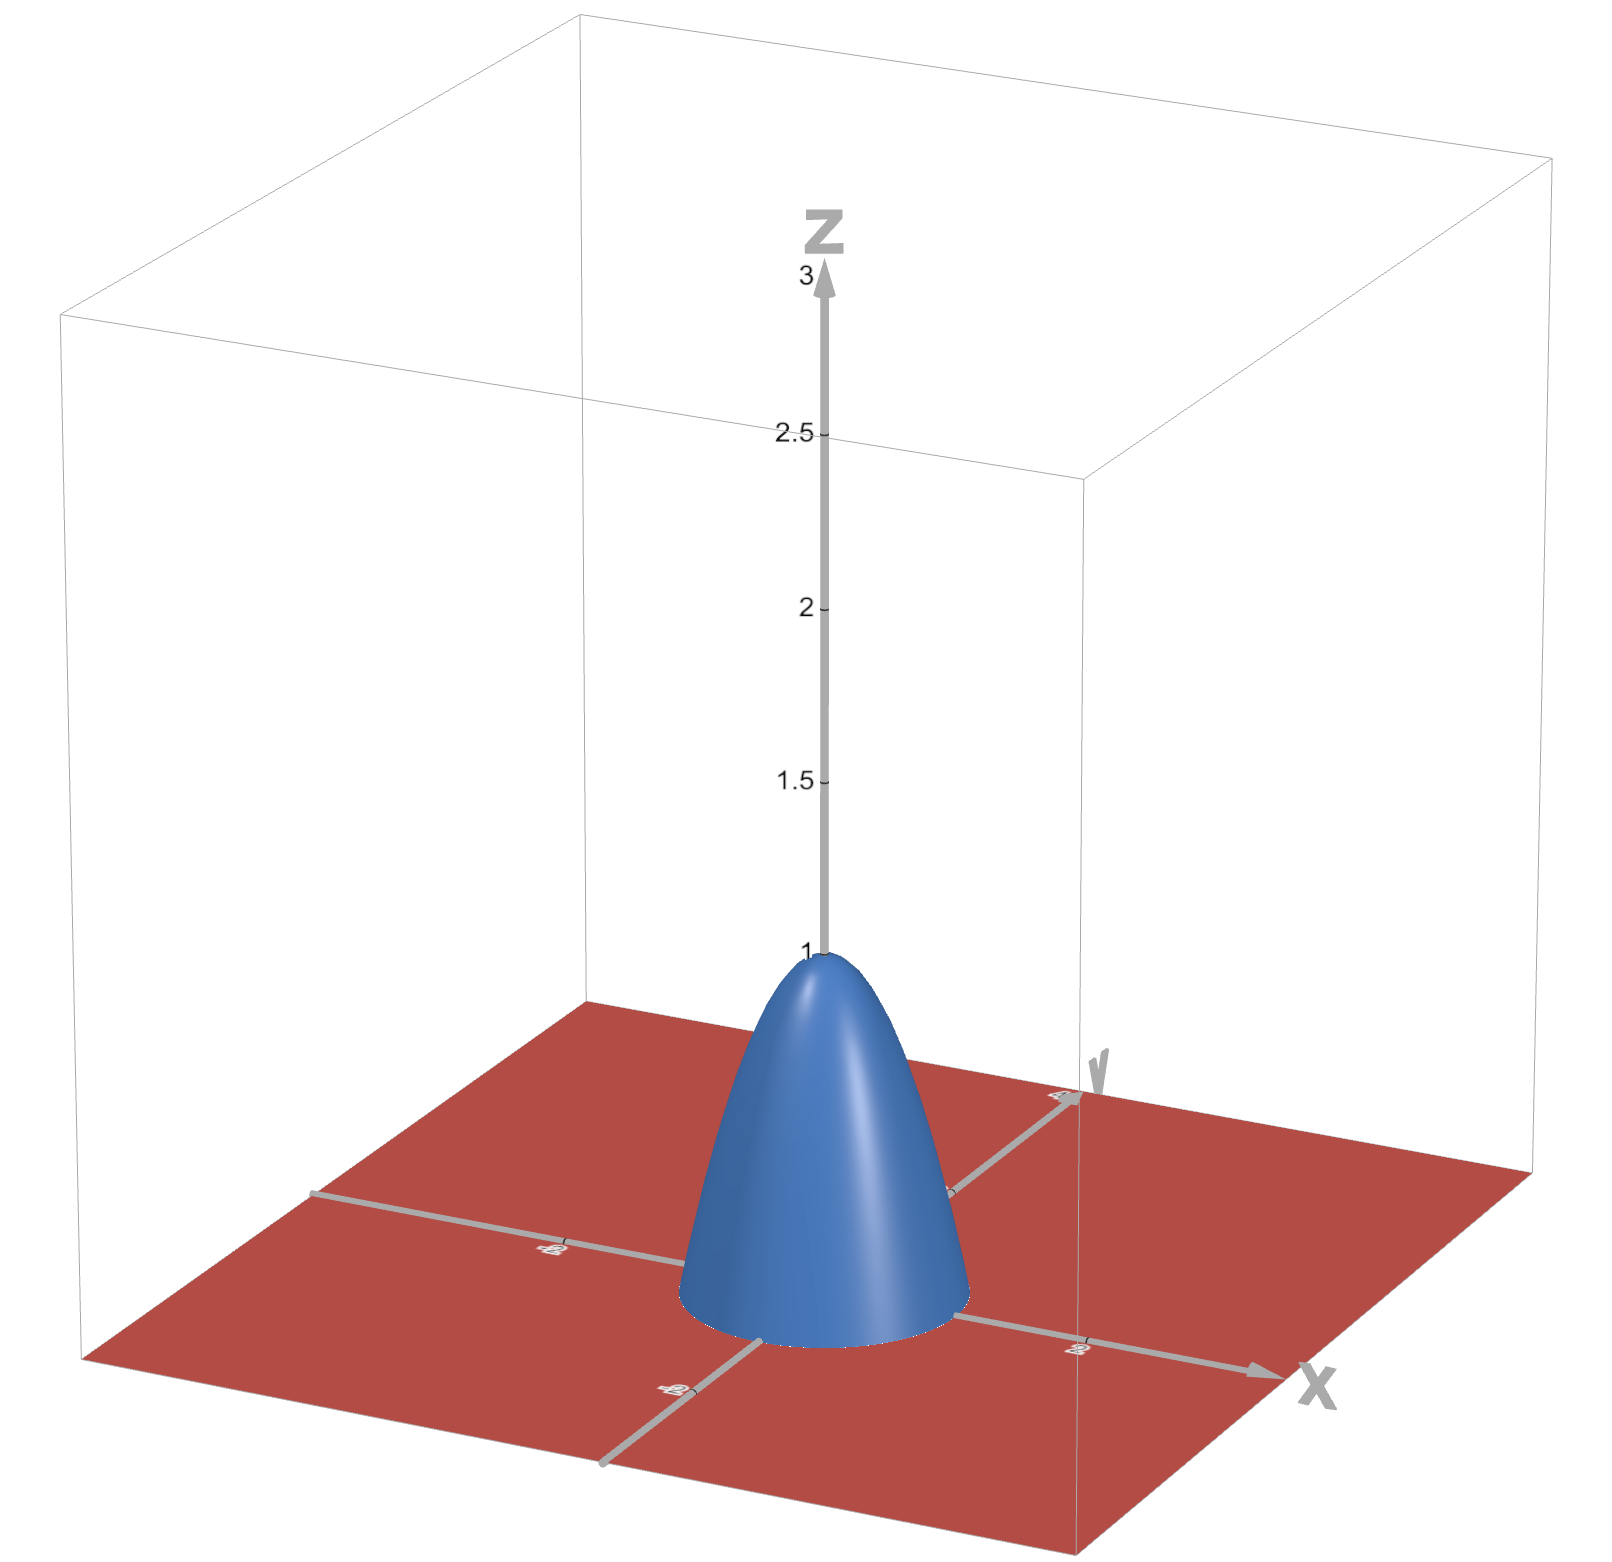
\includegraphics[width=0.40\columnwidth]{./figures/neural_nets//NLA_non_lin_transform.png}
    \caption{The image of our non-linear transformation.}
    \label{fig:non_lin_transformation}
\end{figure}

From here, a natural linear decision boundary is the plane $z=0$ (i.e. the red ground surrounding the blue mountain). Any sample above the plane, i.e. any sample whose $z-$coordinate is positive, is classified as blue. It is otherwise classified as red. We can be more clever than this though. This transformation required us to map samples to 3D — how about mapping to just 1D? To do this, a complete decision function is given by
$$
D(x,y)=\l\lceil\frac{\l\lfloor x^2+y^2\right\rfloor}{x^2+y^2}\right\rceil
$$
and define $D(0,0)=0$ to account for the removable singularity.

\begin{center}
    \textbf{\textcolor{blue}{Q3:} Why not just one activation function in the output layer?}
\end{center}
If there were a single activation function towards the end of the architecture then everything that came before would be a series of linear transformations of the input. The composition of linear transformations is just a linear transformation. As such, the model would effectively be a single linear layer into a non-linear transformation. The only way this could be effective would be if the non-linear transformation were effectively the function we're looking to model in the first place.

\textcolor{red}{note that this is just a single-layer perceptron}: most activation functions are monotonic, so SLPs reduce to, again, a hyperplane in feature space. like the first paragraph states, if we allow for arbitrary non-linear activation functions then this is possbile in theory (but unrealistic). monotonicity kills it

\begin{center}
    \textbf{\textcolor{blue}{Q4:} Must activation functions be monotonic?}
\end{center}
No, it just makes things related to optimisation easier while not impacting performance.

\begin{center}
    \textbf{\textcolor{blue}{Q5:} Which activation functions should be used when?}
\end{center}
Roughly speaking, I wouldn't worry too much about this in practice. They're all nice and differentiable (with small caveats here and there, like with ReLU) allowing for the application of backpropagation. You should sometimes care about the output given the problem at hand. For example, if you need outputs in $[-1,1]$ then $\tanh$ is a natural choice. Note that some choices, like Leaky ReLU, introduce hyperparameters to the model which is sometimes undesirable, e.g. if one seeks a hyperparameterless model.

Small fun note, the universal function approximation of MLPs has been proven only for some select activation functions. I should look in more detail about this.

\begin{center}
    \textbf{\textcolor{blue}{Q6:} Why use a CNN over an MLP?}
\end{center}
Suppose we have an MLP and a CNN, both trained to perform binary classification on images of cats and dogs. Further, suppose they perform equally. It might not be too surprisnig that the MLP will necessarily consist of a number of parameters that is orders of magnitude greater than for the CNN. Also, it's not so clear if a given MLP is translation invariant while various components of a CNN architecture help alleviate fears of translation-related issues.

Also, improved learning-efficiency\footnote{\url{https://ai.stackexchange.com/questions/27407/what-does-statistical-efficiency-mean-in-this-context}}, i.e. fewer samples needed to lean distributions to similar degrees of precision.

% generative models
\section{Deep Generative Models}

Since the era of deep learning began in 2012, tons of generative image, video and text models have arisen. The general idea of these generative models is that if we have a model that fits the data generating process, e.g. the relevant distribution if taking a probabilistic approach, then samples from the model should be sufficiently convincing. That is, if I get a nice fit for the distribution of images of cats lounging in the sun then samples from my fit distirubtion should look convincingly like cats lounging in the sun.

The problem with fitting such a distribution is that it is not at all clear what the distribution function would be. These distributions are complex and generally very hard to get right. Most ways to fit the underlying distribution is to perfrom maximum likelihood in some way. Performing maximum likelihood directly without access to any sort of direct distribution function is pretty hard, so it is often done indirectly. For example, when training a variatioanl autoencoder (VAE), you look to maximise a lower bound of the likelihood. The idea is that if this lower bound is sufficiently tight then maximising it in some sense pushes up the true likelihood, maximising it.

% variational autoencoders
\subsection{Variational Autoencoders (VAEs)}
In \autoref{sec:autoencoders}, autoencoders (AEs) were discussed. Autoencoders are great for data compression/decompression, denoising, interpreting complex models, etc. but we haven't seen yet how we might make use of them for generative tasks, i.e. sampling from the nasty/complex underlying distribution of the data they are trained on. An intuitive first idea is to train a compression/decompression autoencoder, randomly generate points in its latent space and feed them through the decoder, as in \autoref{fig:autoencoder_generation_1}. The outputs of the decoder should be similar to the training data, right? No.

\begin{figure}[ht]
    \centering
    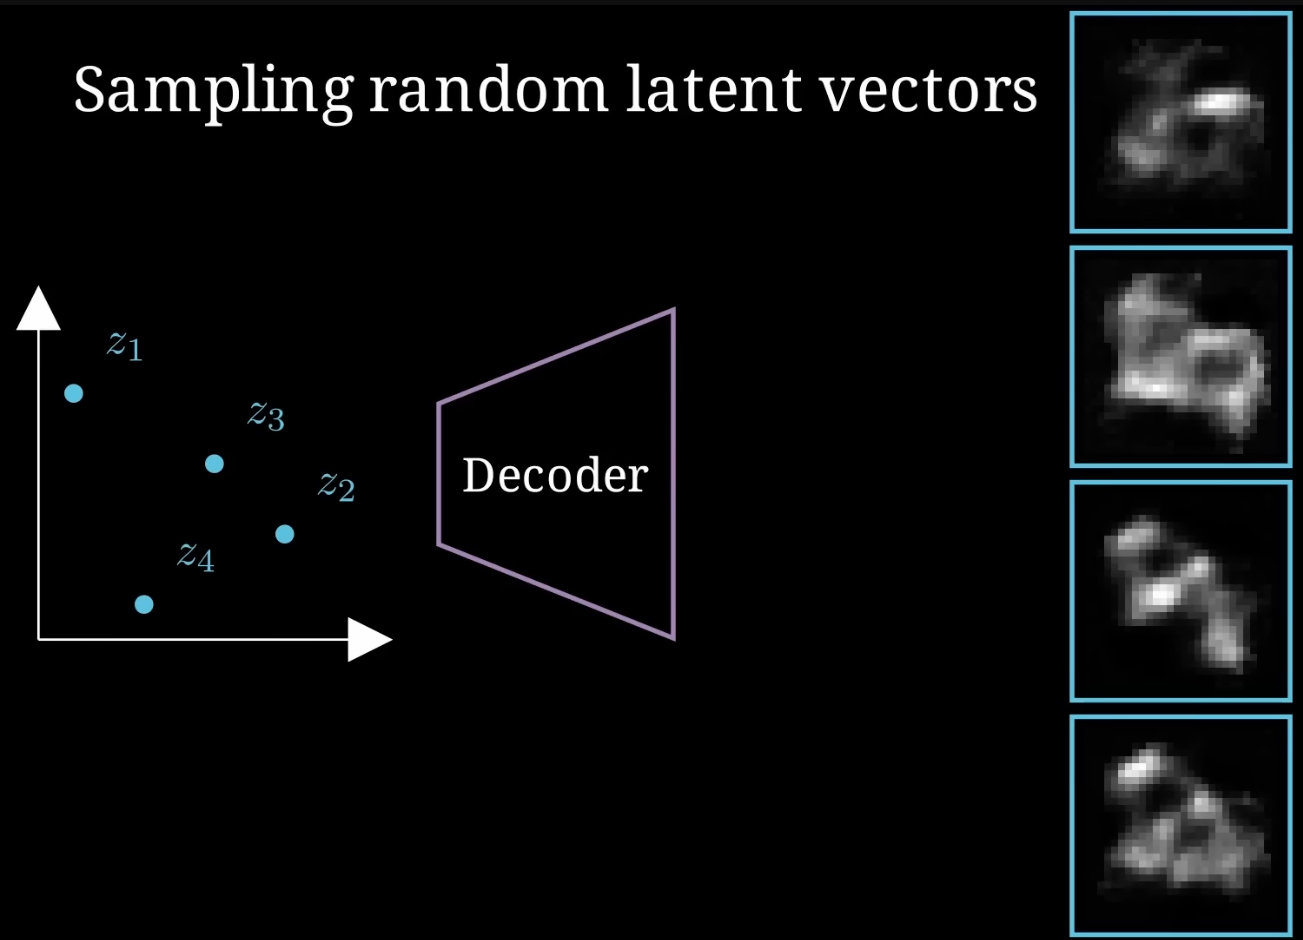
\includegraphics[width=0.60\columnwidth]{./figures/generative_models/AE_gen_1.png}
    \caption{The output of the decoder of an autoencoder with randomly generated latent points as input. Gibberish output.}
    \label{fig:autoencoder_generation_1}
\end{figure}

\noindent Disaster strikes and we begin to see just how unstructured the latent space of an autoencoder is: randomly sampling from it (whatever this may mean) results in nonsense outputs from the decoder because most of the latent space itself is meaningless (nothing is encoded to most of it, so in some sense a lot of it is `un-utilised'). This is perhaps unsurprising as at no point during training an autoencoder do we impose any sort of restriction on the structure of its latent space.

New idea: how about we feed the decoder latent points that are pretty close to the embedding of a given training sample, as in \autoref{fig:autoencoder_generation_2}? This should result in decoder outputs that are similar in structure to the input sample but a bit different, right? No.

\begin{figure}[ht]
    \centering
    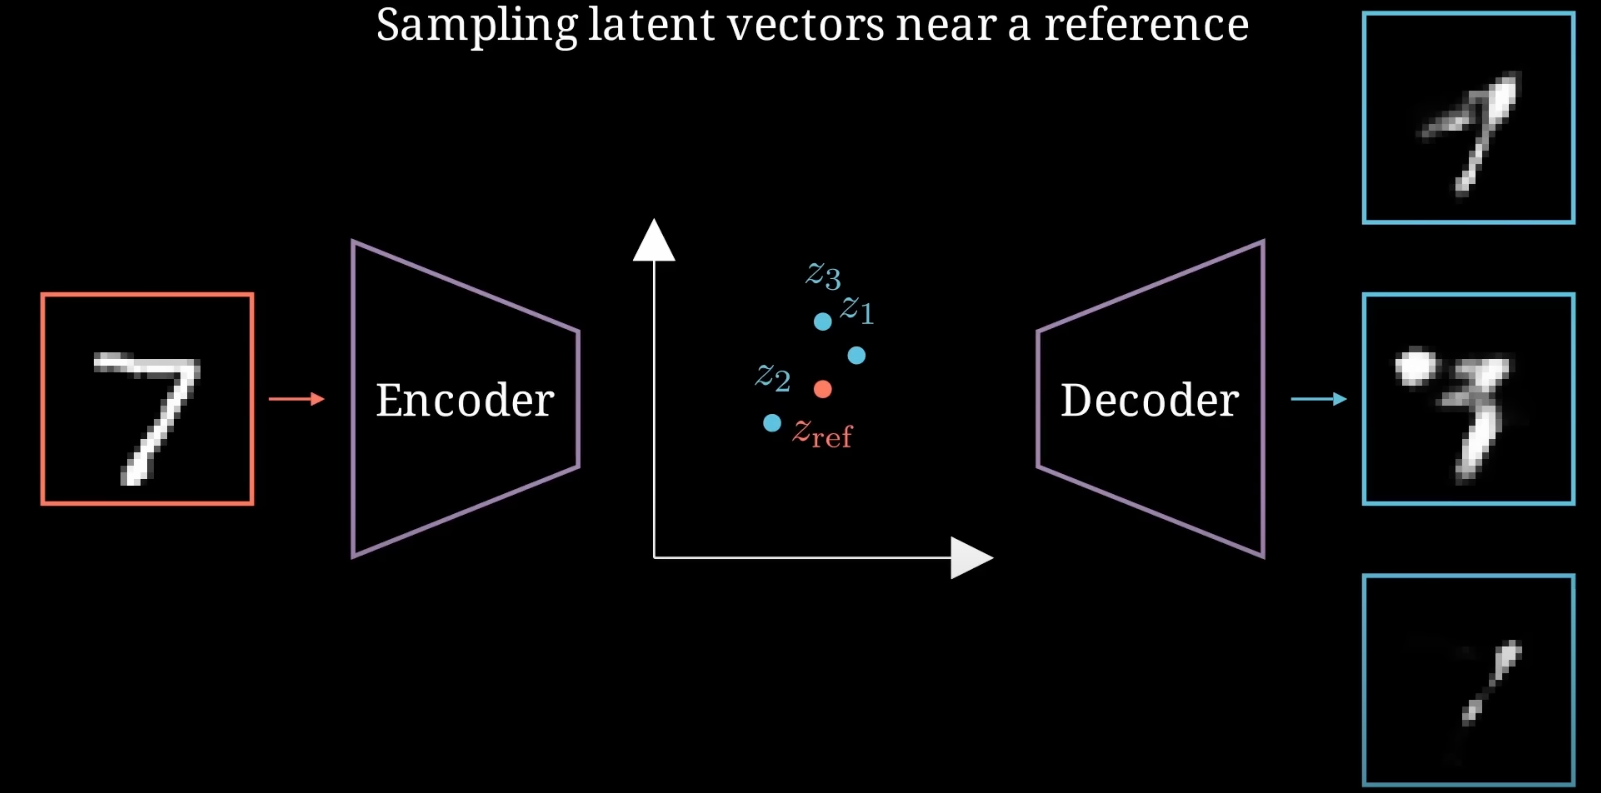
\includegraphics[width=0.75\columnwidth]{./figures/generative_models/AE_gen_2.png}
    \caption{The output of the decoder of an autoencoder points relatively close to the latent embedding of a given training sample.}
    \label{fig:autoencoder_generation_2}
\end{figure}

\noindent Distaster strikes again. To get decoder outputs that are meaningful using this idea, one must take points in the latent space which are ridiculously close to this chosen sample's latent embedding. So close that you'd be practically reconstructing the original training sample each time — certainly not what we mean when we say that we'd like to generate samples.

So how do we do autoencoder-like things in a way that yields well-structured latent spaces? Queue variational autoencoders (VAEs), illustrated in \autoref{fig:VAE_architecture}.

\subsubsection{Formulating VAEs}
Leaving aside, for now, how to learn one from data, VAEs can informally be seen as an extension of autoencoders in which the encoder and decoder each output parameters of a distribution belonging to some pre-chosen distribution family. Extending the notation used to define autoencoders, a variational autoencoder $(\Omega_{\X},d,\mathcal{Q}_d,\mathcal{P}_n,\theta,\phi)$ consists of the sample space of the distribution of interest $\Omega_{\X}\subset\mathbb{R}^n$, a latent dimension $d\in\mathbb{Z}_{\geq1}$, the parameter space $\mathcal{Q}_d$ of a family of $d-$dimensional conditional distributions denoted $q_{\theta}(\z|\x)$, the parameter space $\mathcal{P}_n$ of a family of $n-$dimensional conditional distributions denoted $p_{\phi}(\x|\z)$, an encoder $\theta:\mathbb{R}^n\to\mathcal{Q}_d$ and a decoder $\phi:\mathbb{R}^d\to\mathcal{P}_n$.

To illustrate the intended meaning of the newly-introduced parameter spaces $\mathcal{Q}_d$ and $\mathcal{P}_n$, one's encoder might yield the expectation vector and covariance matrix of a $d-$dimensional Gaussian $\mathcal{N}(\mu,\Sigma)$, i.e. $\mathcal{Q}_d$ could be the parameter space of the family of $d-$dimensional Gaussian distributions yielding
$$
\mathcal{Q}_d
=
\{
(\mu,\Sigma):\mu\in\mathbb{R}^d, \Sigma\in\mathcal{S}_{++}^d
\}
=
\mathbb{R}^d\times\mathcal{S}_{++}^d
$$
where $\mathcal{S}_{++}^d$ denotes the set of all positive-definite matrices in $\mathbb{R}^{d\times d}$.

As the encoder of a VAE yields a $d-$dimensional distribution $q_{\theta}(\z|\x)$ given the sample $\x\in\Omega_{\X}$, to obtain a latent $d-$dimensional representation $\z'\in\mathbb{R}^d$ of $\x$, one computes the parameters $\theta(\x)\in\mathcal{Q}_d$ of $q_{\theta}(\z|\x)$, e.g. a $d-$dimensional Gaussian, via the encoder and samples $\z'\sim q_{\theta}(\z|\x)$. To reconstruct $\x$ from its latent representation $\z'$, one computes the parameters $\phi(\z')\in\mathcal{P}_n$ of the $n-$dimensional reconstruction distribution $p_{\phi}(\x|\z')$ via the decoder. Sampling $\x'\sim p_{\phi}(\x|\z')$ yields (ideally) a sufficiently-accurate reconstruction of the original sample $\x$. Achieving accurate reconstructions is done in a similar manner to autoencoders: by including a penalty term pertaining to reconstruction quality in the loss function used to learn the encoder and decoder.

Note that one's choice of $\mathcal{Q}_d$ and $\mathcal{P}_n$ should take into account the need to sample efficiently and so they should correspond to families of distributions which offer efficient means of sampling, e.g. Gaussians, as in \autoref{fig:VAE_architecture}.

\begin{figure}
    \centering
    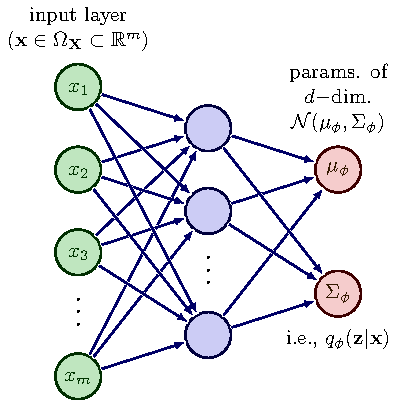
\includegraphics[width=0.46\linewidth]{figures/generative_models/VAE_encoder.pdf}
    \hspace{20pt}
    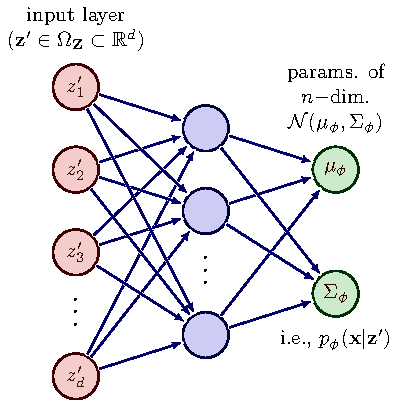
\includegraphics[width=0.46\linewidth]{figures/generative_models/VAE_decoder.pdf}
    \caption{Left: an encoder which outputs parameters of the latent distribution $q_{\theta}(\z|\x)=\mathcal{N}(\mu_{\theta},\Sigma_{\theta})$. Right: a decoder which outputs parameters of the reconstruction distribution $p_{\phi}(\x|\z')=\mathcal{N}(\mu_{\phi},\Sigma_{\phi})$ in which $\z'\sim q_{\theta}(\z|\x)$.}
    \label{fig:VAE_architecture}
\end{figure}

\begin{example}
    Suppose $X_1\sim\mathcal{N}(1,2)$ and $X_3\sim\mathcal{N}(-1,1)$ are independent. Let $X_2=X_1+\epsilon$ where $\epsilon\sim\mathcal{N}(0,1)$ is independent of $X_1$ and $X_3$. If $X=(X_1,X_2,X_3)$ then $X\sim\mathcal{N}(\mu,\Sigma)$ with $\mu=(1,1,-1)'$ and
    $$
    \Sigma
    =
    \begin{bmatrix}
        2 & 2 & 0\\
        2 & 3 & 0\\
        0 & 0 & 1
    \end{bmatrix}.
    $$
    As such, $\Omega_{\X}=\mathbb{R}^3$. To obtain two-dimensional representations of samples $\x\in\Omega_{\X}$ (so $d=2$), one might choose $\mathcal{Q}_2=\mathbb{R}^2\times\mathcal{S}_{++}^2$ and $\mathcal{P}_3=\mathbb{R}^3\times\mathcal{S}_{++}^3$. That is, we could fit a two-dimensional Gaussian to the latent space and a three-dimensional Gaussian to the reconstruction space. Knowing $X_2=X_1+\epsilon$, where $\epsilon\sim\mathcal{N}(0,1)$, one might choose the encoder
    \begin{align*}
        \theta&:
        \Omega_{\X}\to\mathcal{Q}_2\\
        &(x_1,x_2,x_3)\mapsto((x_1,x_3),\sigma^2I_2)
    \end{align*}
    where $\sigma>0$ is small. That is, for a sample $(x_1,x_2,x_3)\in\Omega_{\X}$, the encoder's output would yield the latent distribution $q_{\theta}(\z|\x)=\mathcal{N}((x_1,x_3),\sigma^2I_2)$. As decoder, if all we desire is accurate reconstructions, we might choose
    \begin{align*}
        \phi&:
        \mathbb{R}^2\to\mathcal{P}_3\\
        &(z_1,z_2)\mapsto((z_1,z_1,z_2), \sigma^2I_3).
    \end{align*}
    That is, for the latent sample $\z'=(z_1',z_2')$, the decoder's output would yield the reconstruction distribution $p_{\phi}(\x|\z')=\mathcal{N}((z_1',z_1',z_2'),\sigma^2I_3)$. Ideally, sampling $(x_1',x_2',x_3')\sim p_{\phi}(\x|\z')$ would yield a sample sufficiently similar to the original sample $\x=(x_1,x_2,x_3)$.

    Note that in practice, one does not know the true distribution $p(\x)$ and so hand-picking the encoder and decoder as in this example is infeasible. Typically, the encoder and decoder are learned from a dataset $\mathcal{D}\subset\Omega_{\X}$.
\end{example}
At this point, a natural question arises: for which tasks is learning a VAE more appropriate than learning an autoencoder? The answer lies in the purpose of VAEs which is two-fold: 1) to perform sufficiently-accurate compression/decompression and 2) to produce a sufficiently regularised approximation of the latent space $\Omega_{\Z}$. The latter is ensured by how one learns a VAE from data, which we soon consider. In brief, when learning an autoencoder one never imposes restrictions on the latent space beyond encouraging the model to yield sufficiently-accurate reconstructions. As a result, the latent space of an autoencoder is not well-structured. For example, for latent samples $\z_1,\z_2\in\Omega_{\Z}$ which are `close' in the latent space, their reconstructions are not necessarily `close' in $\mathbb{R}^n$. VAEs seek to remedy this.

To learn a VAE from data, we look to maximise the evidence lower bound (ELBO) over some dataset $\mathcal{D}=\{\x_1,\dots,\x_M\}\subset\Omega_{\X}$. Over a single sample $\x\in\Omega_{\X}$, the ELBO is a tight lower bound of $\log(p(\x))$. As such, maximising the ELBO over $\mathcal{D}$ can be seen as performing approximate maximum-likelihood estimation over $\mathcal{D}$ (sometimes referred to as evidence maximisation). To derive the ELBO, first note that given a decoder $\phi$ (which parameterises the reconstruction distribution $p_{\phi}(\x|\z)$), we may express the marginal distribution $p(\x)$ using $p_{\phi}(\x|\z)$ as
\begin{equation}
\label{eq:marginal_likelihood}
p(\x)
=
\int p(\x,\z)d\z
=
\int p(\x|\z)p(\z)d\z
=
\int p_{\phi}(\x|\z)p(\z)d\z.
\end{equation}
Using \autoref{eq:marginal_likelihood}, along with the encoder $\theta$ (which parameterises the latent distribution $q_{\theta}(\z|\x)$) we derive the ELBO over a single sample $\x\in\Omega_{\X}$:
\begin{align*}
    \log(p(\x))
    &=
    \log\l(\int p_{\phi}(\x|\z)p(\z)d\z\r)\\
    &=
    \log\l(\int q_{\theta}(\z|\x)\frac{p_{\phi}(\x|\z)p(\z)}{q_{\theta}(\z|\x)}d\z\r)\\
    &=
    \log\l(\E_{\Z\sim q_{\theta}(\z|\x)}\l[\frac{p_{\phi}(\x|\Z)p(\Z)}{q_{\theta}(\Z|\x)}\r]\r)\\
    &\geq
    \E_{\Z\sim q_{\theta}(\z|\x)}\l[\log\l(\frac{p_{\phi}(\x|\Z)p(\Z)}{q_{\theta}(\Z|\x)}\r)\r]\\
    &=
    \E_{\Z\sim q_{\theta}(\z|\x)}\l[\log(p_{\phi}(\x|\Z))\r]-\E_{\Z\sim q_{\theta}(\z|\x)}\l[\log\l(\frac{q_{\theta}(\Z|\x)}{p(\Z)}\r)\r]\\
    &=
    \E_{\Z\sim q_{\theta}(\z|\x)}\l[\log(p_{\phi}(\x|\Z))\r]-D_{\text{KL}}(q_{\theta}(\Z|\x)||p(\Z))\\
    &=:
    \text{ELBO}
\end{align*}
in which the inequality arises due to Jensen's inequality, as in $\E[\log(f(\Z))]\leq\log(\E[f(\Z)])$, and $D_\text{KL}(Q||P)$ denotes the KL-divergence between distributions $Q$ and $P$, which is detailed in \textcolor{red}{entropy part?}. The effect of maximising
$$
\text{ELBO}
=
\E_{\Z\sim q_{\theta}(\z|\x)}\l[\log(p_{\phi}(\x|\Z))\r]-D_{\text{KL}}(q_{\theta}(\Z|\x)||p(\Z))
$$
over a dataset is often explained term-by-term. The first term is a principled measure of the VAE's ability to reconstruct latent representations, as with autoencoders. The second term is a principled measure of the similarity of the latent distribution $q_{\theta}(\z|\x)$ and the prior $p(\z)$. The prior is chosen before training and the most common choice is a $d-$dimensional standard Gaussian, i.e. $p(\z)=\mathcal{N}(0,I_d)$. As such, minimising the negative KL-divergence between the latent distribution and said prior is often interpreted as encouraging the learning of the encoder such that latent representations are distributed according to the prior. This is particularly useful in the case that one is learning a VAE to generate new samples from $\Omega_{\X}$: post-training, sample $\z'\sim p(\z)$, compute the parameters $\phi(\z')$ of the reconstruction distribution $p_{\phi}(\x|\z')$ via the decoder and sample from it. Note that using a VAE for generative purposes does not invoke the use of the encoder, only the decoder is required post-training.

Given a dataset $\mathcal{D}=\{\x_1,\dots,\x_M\}\subset\Omega_{\X}$, we learn a VAE by choosing function classes $\Theta$ and $\Phi$ (e.g. MLPs as in \autoref{fig:VAE_architecture}) and computing
$$
\argmax_{(\theta,\phi)\in\Theta\times\Phi}
\l[
\sum_{i=1}^M
\E_{\Z\sim q_{\theta}(\z|\x_i)}\l[\log(p_{\phi}(\x_i|\Z))\r]-D_{\text{KL}}(q_{\theta}(\Z|\x_i)||p(\Z))
\r].
$$
In practice, after choosing a latent dimension $d$, we often take $p(\z)=\mathcal{N}(0,I_d)$, $\mathcal{Q}_d=\mathbb{R}^d\times\mathcal{S}_{++}^d$ and $\mathcal{P}_n=\mathbb{R}^n\times\mathcal{S}_{++}^n$, i.e. Gaussians for the latent and reconstruction distribution families and the standard $d-$dimensional Gaussian for the prior. A benefit of these choices is that it yields a differentiable and easy-to-implement closed form for the KL-divergence term in the ELBO. Additionally, the expectation pertaining to the reconstruction term is typically approximated via a single sample, boiling down to a mean square error term\footnote{\url{https://n8python.github.io/mnistLatentSpace/}}.

\subsubsection{Backpropagation for VAEs}
The expectation term in the ELBO requires us to sample from $q_{\theta}(\z|\x)$. Back propping through sampling is not a thing, it ain't differentiable. We need the reparameterisation trick!

% general adversarial networks
\subsection{Generative Adversarial Networks (GANs)}
Compete!

% normalising flow models
\subsection{Normalising Flow Models}
Turn noise to samples!

% diffusion models
\subsection{Diffusion Models}

\begin{figure}[ht]
    \centering
    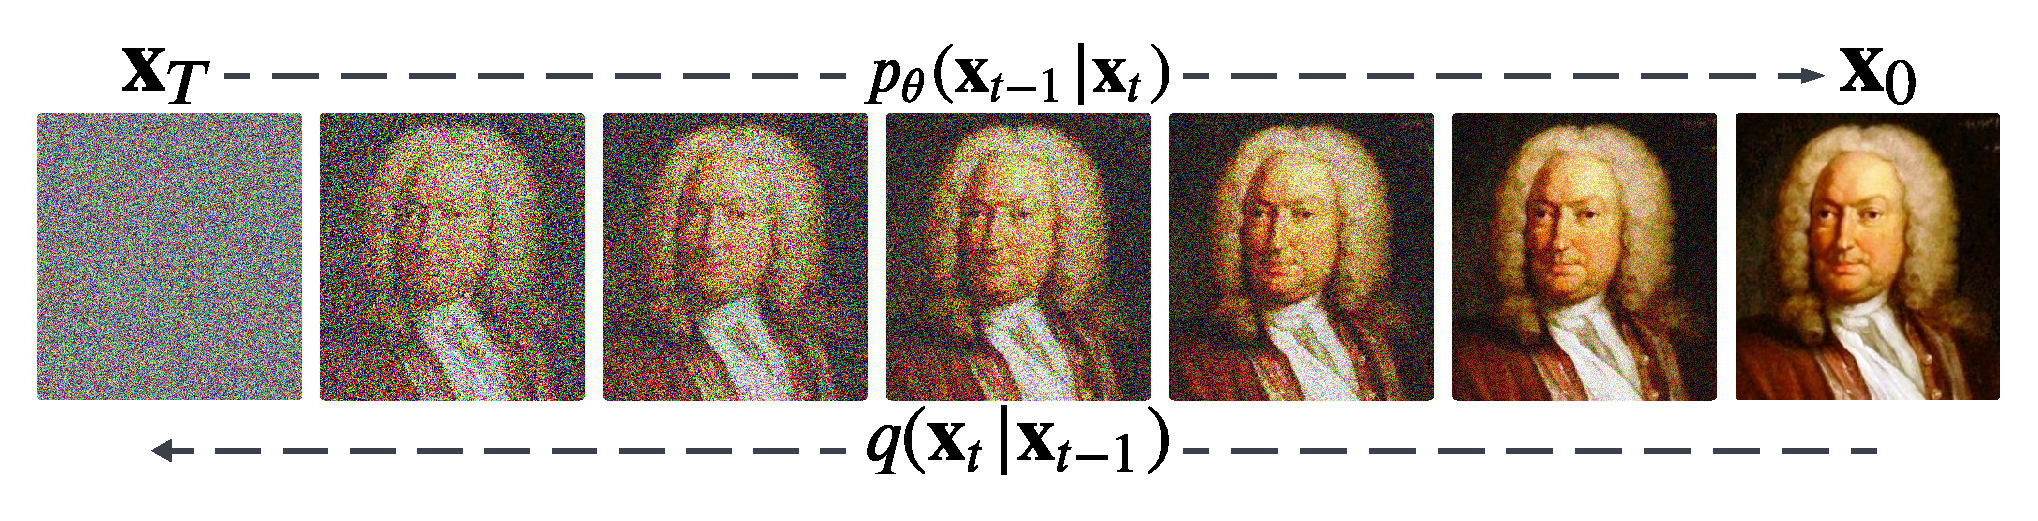
\includegraphics[height=3cm]{./figures/generative_models/diffusion_process.pdf}
    \caption{Johann Bernoulli being denoised in line with the backward process of a diffusion model.}
    \label{fig:diffusion_process}
\end{figure}

The purpose of diffusion models is to facilitate the generation of samples from complex distributions from which sampling is typically intractable. While this overarching motive is not unique to diffusion models, how a diffusion model learns and how it generates new samples is quite distinct from other well-known generative models like VAEs and GANs (though some ideas are certainly comparable). A diffusion model can be described by its forward (noising) and backward (denoising) processes. Its forward process iteratively noises a sample $\x_0\in\mathcal{X}$, belonging to the distribution of interest, $T$-many times to obtain its noised equivalent $\x_T$. Formally, this is done via the Markov process
$$
q(\x_t|\x_{t-1})
=
\mathcal{N}\l(\x_t|\sqrt{1-\beta_t}\x_{t-1},\beta_tI\r)
$$
where $\beta_1,\dots,\beta_T\in[0,1]$ are hyperparameters satisfying $\beta_i<\beta_{i+1}$, often referred to as the noise schedule of the model. With an appropriately chosen final time $T$, these noised equivalents $\x_T$ are akin to random noise sampled from $\mathcal{N}(0,I)$.

Letting $\alpha_t=1-\beta_t$ and $\Bar{\alpha}_t=\prod_{i=1}^t\alpha_i$, we can describe the backward process of a diffusion model again as a Markov process in which we sample some random noise $\x_T$ from $\mathcal{N}(0,I)$ and obtain the $(t-1){\text{st}}$ denoised sample from $p_{\theta}(\x_{t-1}|\x_t)$ via
$$
\x_{t-1}=\frac{1}{\sqrt{\alpha_t}}\l(\x_t-\frac{1-\alpha_t}{\sqrt
{1-\bar{\alpha}_t}}\epsilon_{\theta}(\x_t,t)\r)+\sigma_t\z
$$
where $\sigma_1,\dots,\sigma_T$ are hyperparameters, $\epsilon_{\theta}$ is the diffusion model's denoiser and $\z$ is sampled from $\mathcal{N}(0,I)$. % For clarity, $p_{\theta}(\x_{t-1}|\x_t)=\mathcal{N}(\x_{t-1}|\mu_{\theta}(\x_t,t),\sigma_tI)$ where $\mu_{\theta}(\x_t,t)$ is determined by the decoder $\epsilon_{\theta}$, the current noised image $\x_t$ and the time step $t$.
The purpose of the denoiser $\epsilon_{\theta}$, where $\theta$ is its tuple of parameters, is akin to its name: it is used to iteratively turn sampled noise $\x_T\in\mathcal{N}(0,I)$ into something resembling a sample $\x_0\in\mathcal{X}$ from the distribution of interest. If the architecture of its denoiser can be backpropagated through then training a diffusion model can be done in the usual manner of choosing an appropriate loss function and performing gradient descent in which gradients are computed via backpropagation through the entire model. We leave further details of training a diffusion model out for the sake of brevity but these can easily be found in literature.

So, what is an appropriate choice for the architecture of a diffusion model's denoiser? Before considering transformers for this task, we consider a more often-used choice, U-Net: a class of convolutional neural networks (CNNs).

\subsection{U-Net denoisers}
Despite not being the choice of denoiser made in the seminal paper introducing diffusion models, U-Net became the go to choice of denoiser architecture for contemporary diffusion models. To understand U-Net's popularity in this regard, it is worth understanding its architecture which consists of a contracting branch, terminating at its bottleneck, followed by an expansion branch, illustrated in \autoref{fig:u_net_arch}. This architecture can be thought of as forming a `U'-like shape, with the bottleneck lying at the bottom, hence its name.

\begin{figure}[ht]
    \centering
    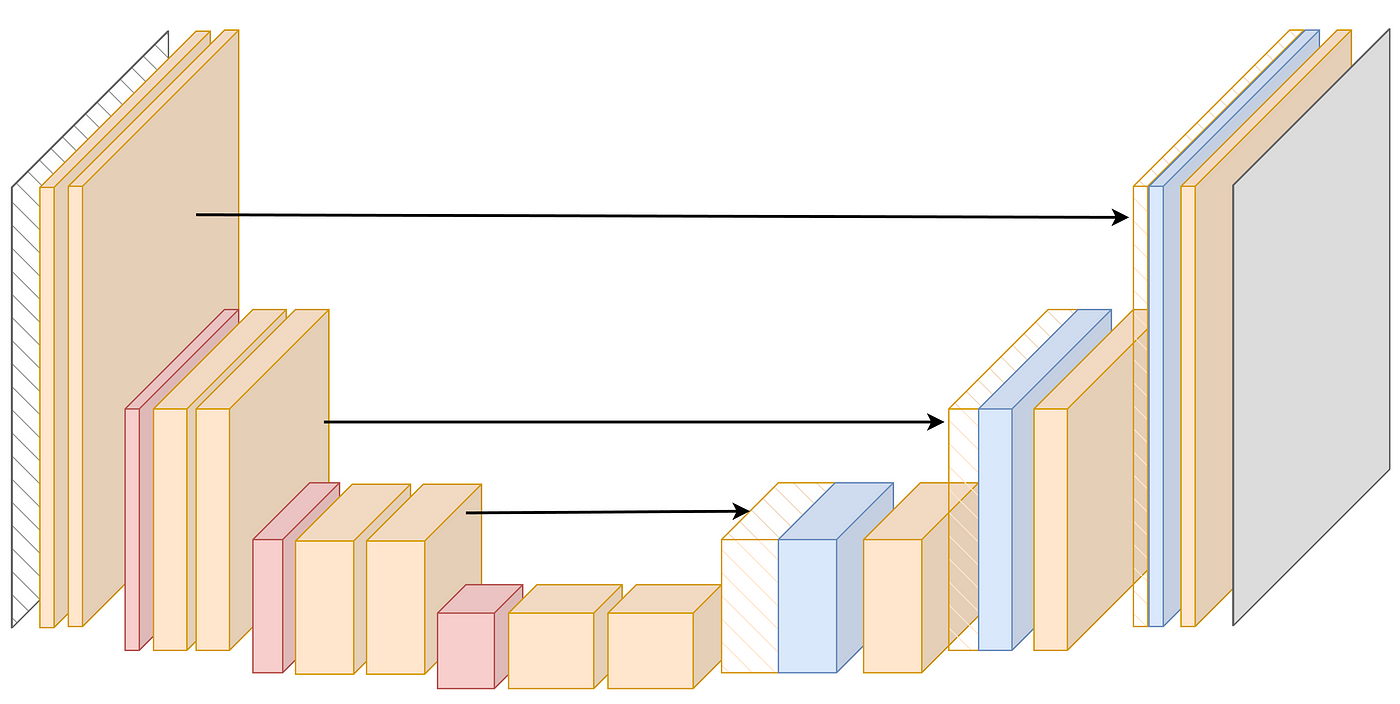
\includegraphics[width=\columnwidth]{./figures/generative_models/unet.png}
    \caption{\centering Example U-Net architecture.}
    \label{fig:u_net_arch}
\end{figure}

\noindent In the context of denoising, the contraction branch takes a noised image as input and iteratively completes a series of convolution operations followed by max pooling until reaching the bottleneck layer. At the bottleneck, the model has heavily reduced the spatial dimension of the input image while extracting varying levels of feature abstractions. For example, after the first iteration of convolution and max pooling, the spatial dimension of the input image may be reduced from $1024\times1024$ to $512\times512$ but edges and textures within the original image may be encoded in the feature maps at this stage. Then, during expansion, the model looks to upscale from the bottleneck in a way that retains the underlying image while removing noise. This is done by iteratively completing a series of deconvolutions, which correspond to upscaling, and using skip connections from its corresponding component in the contraction branch, seen in \autoref{fig:u_net_arch}, in order to retain the underlying image. With this in mind, it is clear why U-Net has been the go to choice of denoiser when developing a diffusion model.

% transformer models
\subsection{Transformers}
Stand at attention!

\subsubsection{Token embedding}
Embed the semantics of tokens in high-dimensional space:
$$
E(\text{Germany})
+E(\text{fascist})
-E(\text{Mussolini})
\approx
E(\text{Hitler}).
$$
So the embedding function $E$ maps from the token vocabulary $S$ to some high-dimensional space. If you first encode the tokens in the token vocabulary, e.g. via enumeration, then
$$
E:\{1,\dots,|S|\}\to\mathbb{R}^d
$$
where $d\in\mathbb{N}\backslash\{0\}$ is the embedding dimension. What makes token embedding functions interesting is how well they can capture semantics of language.

\subsubsection{Positional encoding}
Use sinusoids to form a position vector $P_k$ for the $k$th token in an input sequence of length $L$. Add $P_k$ to the word embedding $E_k$ for $k=0,\dots,L-1$ to obtain the input $[E_0+P_0,\dots,E_{L-1}+P_{L-1}]$ fed to the model.

% misc. questions
\addtocontents{toc}{\protect\setcounter{tocdepth}{1}}
\subsection{Misc. questions}
\addtocontents{toc}{\protect\setcounter{tocdepth}{2}}

Some questions to challenge one's understanding.

\begin{center}
    \textbf{\textcolor{blue}{Q1:} Blelele?}
\end{center}
\dots

% object detection models
\section{Object Detection Models}

CNNs and transformer-based architectures have revolutionised object detection. Three main flavours: R-CNN, YOLO and DETR. Before going into detail about them, what is object detection? What methods came before CNN/transformer-based architectures?

% R-CNN
\subsection{(Fast/Faster) R-CNN}
R-CNN models has three flavours: R-CNN, Fast R-CNN and Faster R-CNN. R-CNN stands for \textit{Regions with CNN features}. Roughly put, detecting objects within a given image using an R-CNN model consist of two parts:
\begin{enumerate}
    \item Proposing regions of interest within the image
    \item Classifying what is in each region (if there is something in the region)
\end{enumerate}

% appendices
\newpage
\begin{appendices}
\addtocontents{toc}{\protect\setcounter{tocdepth}{0}}

% probability things
\section{Probability Theory Things}

\begin{tcolorbox}[colback=c5]
    \textbf{Discrete:}
    \begin{itemize}
        \item Bernoulli $\rightarrow$ Binomial \textbf{(binary classification)}
        \item Categorical $\rightarrow$ Multinomial \textbf{(multi-class classification)}
    \end{itemize}
\end{tcolorbox}

\begin{tcolorbox}[colback=c9]
    \textbf{Continuous:}
    \begin{itemize}
        \item (Multivariate) Normal \textbf{(generic)}
    \end{itemize}
\end{tcolorbox}

\subsection{From Bernoulli to Binomial}
Let's try to generalise the Bernoulli distribution to the binomial distribution. If $X\sim\text{Ber}(p)$ then $\Omega_X=\{0,1\}$ and $\P(X=x)=p^x(1-p)^{1-x}$, so $\P(X=1)=p$ and $\P(X=0)=1-p$.

Taking $n$ independent Bernoulli trials and summing them yields the random variable $\X=\sum_{i=1}^nX_i\sim\text{Bin}(n,p)$ with $\OX=\{0,\dots,n\}$. Let $k$ denote a realisation of $\X$, i.e. $k=x_1+\dots+x_n$. The corresponding mass function is given by
\begin{align*}
    \P(\X=k)
    &=
    Z\cdot\prod_{i=1}^n\P(X_i=x_i)\\
    &=
    Z\cdot\prod_{i=1}^np^{x_i}(1-p)^{1-x_i}\\
    &=
    Z\cdot p^{x_1+\dots+x_n}(1-p)^{n-(x_1+\dots+x_n)}\\
    &=
    Z\cdot p^k(1-p)^{n-k}
\end{align*}
where $Z$ is a normalising constant accounting for the number of ways one can permute the tuple of realisations $(x_1,\dots,x_n)\in\Omega_{X}^n$. So $Z$ is just the number of ways of placing $k$-many $1$s among a series of $n>k$ digits, i.e. $Z=\binom{n}{k}$, so
$$
\P(\X=k)
=
\binom{n}{k}p^k(1-p)^{n-k}.
$$

\subsection{From Categorical to Multinomial}
The categorical distribution is a generalisation of the Bernoulli distribution and the multinomial distribution is a generalisation of the binomial distribution. In line with this, we'd hope to be able to generalise the categorical distribution to the multinomial distribution.

If $X\sim\text{Cat}(p_1,\dots,p_C)$ then realisations of $X$ can be represented by single integers in $\{1,\dots,C\}$ but I prefer to represent them in terms of their $C-$long one-hot encodings. So I denote the presence of the $c^{\text{th}}$ class in a realisation as the unit row vector $\mathbf{e}_c^{\text{T}}$, e.g. $(0,1,0\dots,0)$ denotes a sample in which only the second class is present. The corresponding mass function is then given by
$$
\P(X=(x_1,\dots,x_C))
=
\prod_{j=1}^Cp_j^{x_j}.
$$
Note that, in this notation, all but one of these $x_j$ terms are zero, so it really boils down to just a single probability value, e.g. $\P(X=(0,1,\dots,0))=p_2$. The mass function can also be written using indicator functions but the form offered above is easiest to understand for me.

Applying the same idea used to generalise Bernoulli to binomial, consider the random variable $\X=\sum_{i=1}^nX_i$ pertaining to $n$ independent categorical trials. Each realisation of $X_1,\dots,X_n$ can be represented by a $C-$long one-hot encoded vector and so $n$ realisations of $X\sim\text{Cat}(p)$ can be thought of as a matrix $\x\in\{0,1\}^{n\times C}$ whose rows are unit vectors in $\R^C$. As such, letting $k_1,\dots,k_C$ denote the number of $1$s in the columns of $\x$ (so $k_1+\dots+k_C=n$) we see immediately that $(k_1,\dots,k_C)$ is a realisation of $\X$. So what is the corresponding mass function? Let $x_{ij}$ denote the element in the $i^{\text{th}}$ row and $j^{\text{th}}$ column of $\x$ and let $k_j=x_{1j}+\dots+x_{nj}$ denote the sum of all elements in the $j^{\text{th}}$ column of $\x$. Note that $k_j$ is the number of realisations of $X_1,\dots,X_n$ in which the $j^{\text{th}}$ class is present. We have
\begin{align*}
    \P(\X=(k_1,\dots,k_C))
    &=
    Z\cdot\prod_{i=1}^n\P(X_i=(x_{i1},\dots,x_{iC}))\\
    &=
    Z\cdot\prod_{i=1}^n\prod_{j=1}^Cp_j^{x_{ij}}\\
    &=
    Z\cdot\prod_{j=1}^Cp_j^{x_{1j}+\dots+x_{nj}}\\
    &=
    Z\cdot\prod_{j=1}^Cp_j^{k_j}\\
    &=
    Z\cdot p_1^{k_1}\cdots p_C^{k_C}.
\end{align*}
So all that's left to do is derive the normalisation constant $Z$. Note that the realisation $\x$ has $n$ rows of which there are $n!$-many orderings. Additionally note that for each $j\in\{1,\dots,C\}$ we know that there are $k_j$-many $1$s in column $j$ so $k_1$ of these $n$ rows must pertain to the first class for which there are $\binom{n}{k_1}$-many orderings. From here, see that $k_2$ of the $n-k_1$ remaining rows must pertain to the second class for which there are $\binom{n-k_1}{k_2}$-many orderings. Continuing this line of reasoning, we obtain
\begin{align*}
    Z
    &=
    \prod_{i=1}^C\binom{n-\sum_{j=1}^{i-1}k_j}{k_i}\\
    &=
    \binom{n}{k_1}\binom{n-k_1}{k_2}\binom{n-(k_1+k_2)}{k_3}\cdots\binom{n-(k_1+\dots+k_{C-1})}{k_C}\\
    &=
    \frac{n!}{k_1!}\cdot\frac{(n-k_1)!}{k_2!(n-(k_1+k_2))!}\cdot\frac{(n-(k_1+k_2))!}{k_3!(n-(k_1+k_2+k_3))!}\cdots\frac{k_C!}{k_C!0!}\\
    &=
    \frac{n!}{k_1!\cdots k_C!}
\end{align*}
from which we obtain
$$
\P(\X=(k_1,\dots,k_C))
=
\frac{n!}{k_1!\cdots k_C!}p_1^{k_1}\cdots p_C^{k_C}.
$$

\subsection{Negative Binomial and Geometric}
We keep flipping our (maybe biased) coin until we observe $r$ successes ($r$ is a parameter) where individual trials are Ber$(p)$ distribured. So if $X\sim\text{NB}(r,p)$ then
$$
\P(X=k)
=
Z\cdot p^r(1-p)^k.
$$
An assignment must be of the form $(x_1,\dots,x_{k+r-1},1)$ which means that $r-1$ of the first $k+r-1$ elements must be a success of which there are $\binom{k+r-1}{r-1}$ possibilities, thus
$$
\P(X=k)
=
\binom{k+r-1}{r-1}p^r(1-p)^k.
$$
The case $r=1$ yields the shifted geometric distribution, whose PMF is just
$$
\P(X=k)
=
p(1-p)^k.
$$

\subsection{The Law of Large Numbers}
Suppose you have some i.i.d. samples $x_1,\dots,x_n\sim p(x)$ then
$$
\frac{1}{n}\sum_{i=1}^n x_i
\xrightarrow{n\to\infty}
\E[X]
$$

\subsection{Entropy}
The entropy of a random variable can be motivated by the notion of the surprise of (or information learned from) observing assignments of said random variable. Given a discrete random variable $X$, an event $E\in\Omega_X$ and a surprise function $S:\Omega_X\rightarrow[0,\infty)$, the surprise of observing $E$ is $S(E)$. Before we continue, we need to understand what we want out of our surprise function. Following the use of `surprising' in day-to-day communication, we want events with low probability to be highly surprising and events with high probability to be less surprising, with some extra conditions. So if $\P(E)=0.01$ then we want $S(E)$ to be close to relatively high (strictly speaking it doesn't need to be bounded above) and if $\P(E)=0.99$ then we want $S(E)$ to be close to 0.

An easy way to achieve this is to take $S(E)=\log(\P(E))$ where $\log$ denotes the natural logarithm. Doesn't really matter which base tbh. Quickly see that $\log(0.01)=4.61$ and $\log(0.99)=0.01$. From here, we define the entropy of a random variable as its expected surprise
$$
H(X)
=
\E[-\log(\P(X))]
=
-\sum_{x\in \Omega_X}\P(x)\log(\P(x)).
$$

\noindent More precisely, Claude Shannon wanted such a surprise function to satisfy three intuitive properties. Firstly, the surprise of an event with probability $1$ should be $0$. Secondly, the surprise of two independent events occurring should be the sum of the surprises of the events individually. Thirdly, the surprise of a given event should be higher than the surprise of any less probable event. So, for all $E_1,E_2\in\Omega_X$, $S:\Omega_X\rightarrow[0,\infty)$ must satisfy
\begin{itemize}
    \item $S(1)=0$
    \item $\P(E_1,E_2)=\P(E_1)\cdot\P(E_2)\implies S(E_1,E_2)=S(E_1)+S(E_2)$
    \item $\P(E_1)>\P(E_2)\implies S(E_1)<S(E_2)$
\end{itemize}

\noindent It's straightforward to see that $S(E)=-\log(\P(E))$ satisfies these three properties but it turns out that it is unique in satisfying these properties, up to its base.\\

\noindent\textbf{Note 1:} It's clear from the second condition that this surprise function is actually a function whose domain is the powerset of $\Omega_X$ but addressing this detail isn't worth it — the idea being conveyed is hopefully clear regardless.\\

\noindent\textbf{Note 2:} You can see entropy as pertaining to a random variable or of a distribution of said random variable. I should formalise this at some point.

\subsubsection{Kullback–Leibler Divergence (KL-divergence)}

Given probability density/mass functions $p$ and $q$ on the same space $\Omega$, their Kullback–Leibler divergence (KL-divergence) is given by
$$
D_{\text{KL}}(p||q)
=
\E_{X\sim p}\left[\log\left(\frac{p(X)}{q(X)}\right)\right].
$$
It is often used as a measure of similarity between two distributions: it follows from Gibbs' inequality that it is non-zero and it is often proposed as a loss function when assessing how well a model $q$ encodes an underlying distribution $p$.

The KL-divergence of two distributions can be expressed in terms of self-entropy and cross-entropy terms as
\begin{align*}
    D_{\text{KL}}(p||q)
    &=
    \E_{X\sim p}\left[\log\left(\frac{p(X)}{q(X)}\right)\right]\\
    &=
    \E_{X\sim p}\left[-\log(q(X))\right]-\E_{X\sim p}\left[-\log(p(X))\right]\\
    &=
    H(p,q)-H(p)
\end{align*}
where $H(p,q)$ denotes the cross-entropy between $p$ and $q$ while $H(p)$ denotes the self-entropy of $p$. It follows that minimising the KL-divergence $D_{\text{KL}}(p,q)$ in $q$ corresponds to minimising the cross-entropy $H(p,q)$.

\subsubsection{Distribution fitting using cross-entropy}
\label{subsubsec:dist_fit_CE}

Suppose we have the geometric distribution with $p=1/2$ and would like to fit it using a Poisson distribution. That is, we would like to best approximate
\begin{align*}
    p:\mathbb{N}\backslash\{0\}&\to[0,1]\\
    k&\mapsto2^{-k}
\end{align*}
by finding a nice $\lambda$ for
\begin{align*}
    q:\mathbb{N}\backslash\{0\}&\to[0,1]\\
    k&\mapsto\frac{e^{-\lambda}\lambda^k}{k!}.
\end{align*}
To find a good $\lambda$, it makes sense to first come up with a metric for how good a given value is. For this, we can use the cross-entropy of the distributions $p$ and $q$ given by
$$
H(p,q)
=
-\E_{K\sim p}\l[\log(q(K))\r]
=
-\sum_{k=1}^{\infty}p(k)\log(q(k))
$$
which can be seen as the incurred cost of using the model $q$ in place of the true underlying model $p$. There are a bunch of different ways of describing/interpreting this quantity. The most interesting is perhaps the one related to encodings. Anyway, in our case, if we can find a closed form of this expression in terms of $\lambda$ then we can look to compute which value of $\lambda$ it's minimised by. In line with this, we compute
\begin{align*}
    H(p,q;\lambda)
    &=
    -\E_{K\sim p}\l[\log(q(K))\r]\\
    &=
    -\sum_{k=1}^{\infty}p(k)\log(q(k))\\
    &=
    -\sum_{k=1}^{\infty}2^{-k}\l(-\lambda+k\log(\lambda)-\log(k!)\r)\\
    &=
    \lambda\sum_{k=1}^{\infty}\frac{1}{2^k}-\log(\lambda)\sum_{k=1}^{\infty}\frac{k}{2^k}+\sum_{k=1}^{\infty}\frac{\log(k!)}{2^k}\\
    &=
    \lambda-\log(\lambda)+C
\end{align*}
where $C=\sum_{k=1}^{\infty}\frac{\log(k!)}{2^k}$ is independent of $\lambda$. In computing the minmum of $H(p,q;\lambda)$ in $\lambda$ we compute
$$
\frac{\partial}{\partial \lambda}H(p,q;\lambda)
=
1-\frac{1}{\lambda}
$$
which yields $\lambda=1$. So according cross-entropy, the best-fitting Poisson distribution to our geometric distribution is Poi$(1)$. For $\lambda=1$ we compute a cross-entropy of
$$
H(p,q;1)
=
1+\sum_{k=1}^{\infty}\frac{\log(k!)}{2^k}
\approx
2.01567.
$$
On its own, this quantity isn't too useful. To get a sense of goodness-of-fit we desire the KL-divergence, i.e. the cross-entropy minus the self-entropy of $p$. Let's compute said self-entropy:
\begin{align*}
    H(p)
    &=
    -\sum_{k=1}^{\infty}p(k)\log(p(k))\\
    &=
    -\sum_{k=1}^{\infty}2^{-k}\log(2^{-k})\\
    &=
    \log(2)\sum_{k=1}^{\infty}\frac{k}{2^k}\\
    &=
    2\log(2)\\
    &\approx
    1.386
\end{align*}
from which we know that the KL-divergence between the underlying geometric distribution $p$ and our Poisson fit $q$ is given by
$$
\text{KL}(p||q)
\approx
2.016-1.386
=
0.63
$$
which seems pretty low. Good fit!

\subsubsection{Distribution fitting using maximum likelihood estimation}
Suppose instead of knowing the nice geometric distribution from \autoref{subsubsec:dist_fit_CE} we only had $n$ i.i.d. samples drawn from it denoted $\D=(k_1,\dots,k_n)\in\mathbb{N}^n$. The MLE of the `true' $k$ of $\text{Poi}(k)$ is given by
$$
k_{\text{MLE}}
=
\frac{1}{n}\sum_{i=1}^n k_i.
$$
The reason I write `true' in the previous sentence is that of course we know that these samples were not drawn from a Poisson distribution at all. This is a nice example of imperfections in model assumptions. Is a Poisson distribution what gave rise to our samples? Is the class of functions given by an MLP with a fixed number of layers and nodes in each layer the function that gave rise to our samples? We're not god afterall.

Anyway, by the law of large numbers, we know that
$$
k_{\text{MLE}}\xrightarrow{n\to\infty}\E[K]=1.
$$
From what I understand, the fact that minimising cross-entropy yields the same estimate as MLE with $n\to\infty$ here is a special case of things learned in generalised linear models. Some sort of result about distributions from exponential families. Sadly, I never took the GLMs course at my university by Wim Krijnen so it isn't obvious to me.

\subsection{The Central Limit Theorem (CLT)}
\dots

% statistics things
\section{Classical Statistics Things}

\subsection{Independent samples}
Suppose we'd like to get an idea of the average height of men and women in our population. If we randomly sample 100 men and 100 women then we're good to go: we have independent samples. If instead we randomly sample 100 couples then our samples would not be independent since couples' heights correlate.

This is important because when performing maximum likelihood, the assumption of independence of samples is key to writing the likelihood of the set as a product of individual probabilities. Without this independence, the likelihood would be a horribly complex function that we would not be able to utilise. Independence is also assumed in a ton of other statistics-related things like t-tests, ANOVA, etc.

\end{appendices}

\end{document}
